\documentclass[journal,a4paper,onecolumn]{IEEEtran}

\usepackage{graphicx}
\usepackage{url}
\usepackage{amsmath}
\usepackage{booktabs}
\usepackage{longtable}
\usepackage{array}
\usepackage{enumitem}
\usepackage{xcolor}
\usepackage{hyperref}
\usepackage{float}

\graphicspath{{diagrams/}{assets/media/}}
\hypersetup{colorlinks=true,linkcolor=blue,urlcolor=blue,citecolor=blue}
\setlength{\LTpre}{4pt}
\setlength{\LTpost}{4pt}
\newcommand{\HRule}{\rule{\linewidth}{0.5mm}}
\newcommand{\req}[1]{\textbf{#1}}

\begin{document}
\begin{titlepage}
\center
~\\[0.5cm]
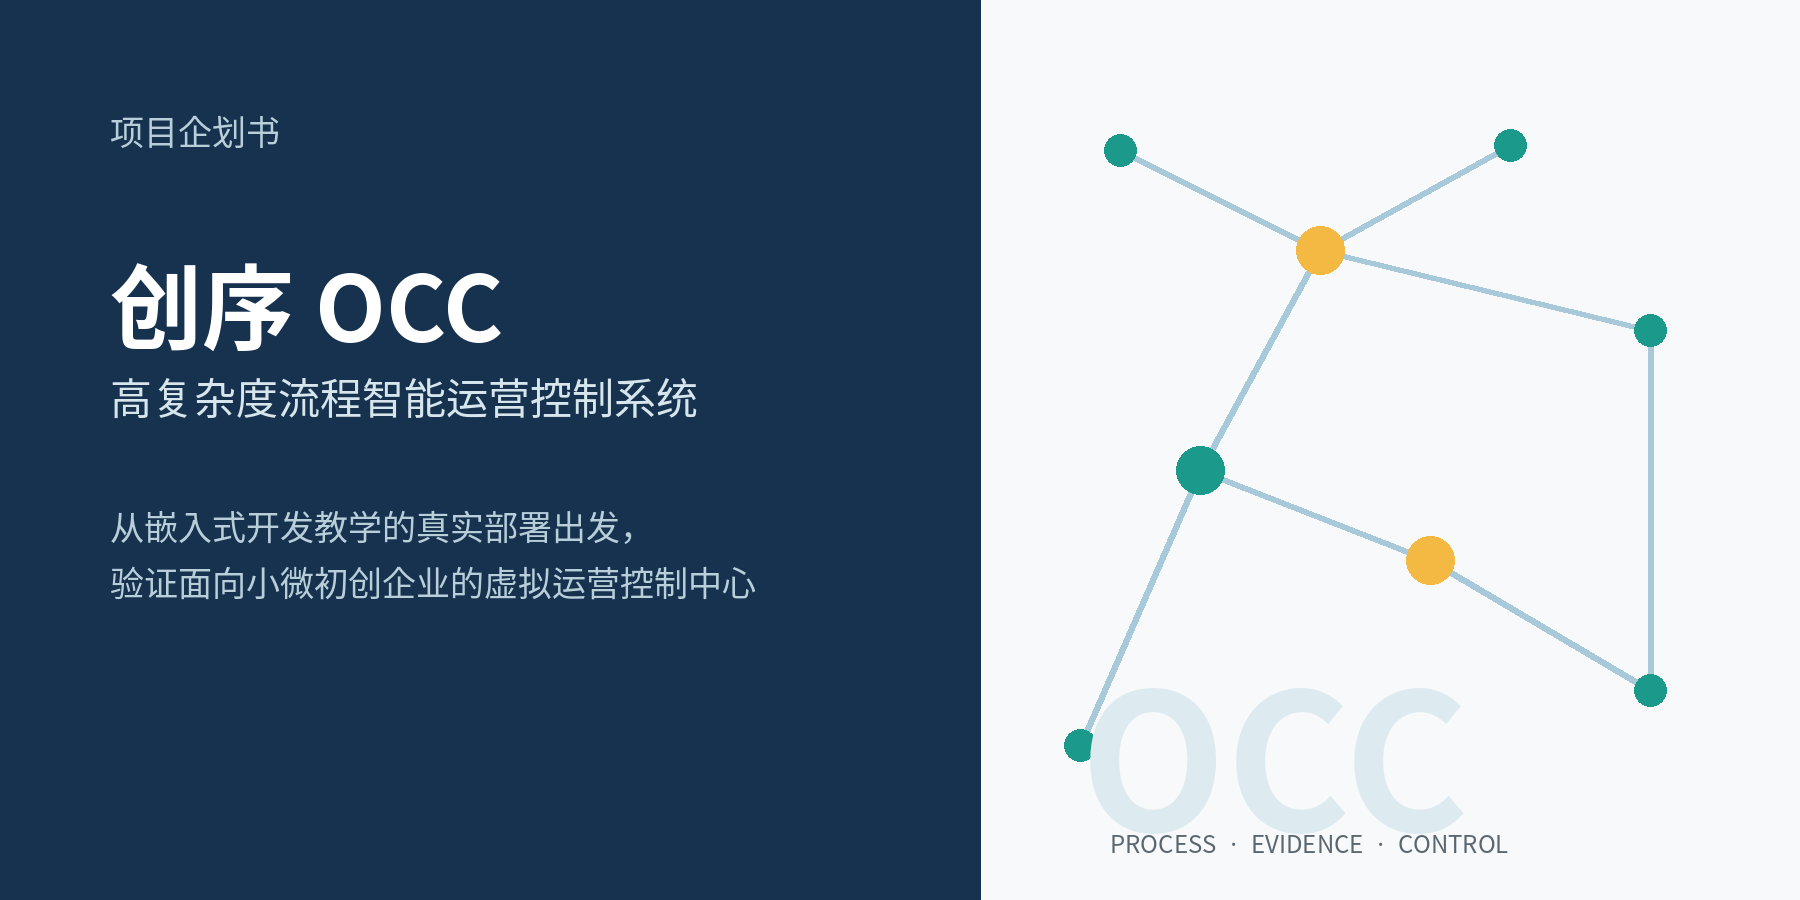
\includegraphics[width=0.88\textwidth]{image1.png}\\[1.0cm]
\HRule \\[0.6cm]
{\huge\bfseries Innorder OCC Software Specification}\\[0.3cm]
{\Large and Database Design}\\[0.6cm]
\HRule \\[1.2cm]
\textsc{\Large Document Language: English}\\[0.5cm]
\textsc{\Large Baseline: 16-week MVP and domain expansion}\\[1.2cm]
\begin{minipage}{0.42\textwidth}
\begin{flushleft}\large
\emph{System:}\\
Innorder OCC
\end{flushleft}
\end{minipage}
\begin{minipage}{0.42\textwidth}
\begin{flushright}\large
\emph{Document version:}\\
1.0
\end{flushright}
\end{minipage}\\[1.2cm]
{\large Prepared: 2026-07-28}\\[0.5cm]
{\large Status: Design baseline / pre-implementation specification}\\[1cm]
\vfill
\end{titlepage}

\title{Innorder OCC: Software Specification and Database Design}
\author{Innorder OCC Project Documentation}
\maketitle

\begin{abstract}
This specification consolidates the Innorder OCC project proposal, approved architecture design, database design, eight executable PostgreSQL/Flyway migrations, and their contract tests. It defines product scope, functional requirements, architecture boundaries, domain semantics, critical transactions, security controls, non-functional requirements, and the physical database design. Innorder OCC separates a deterministic workflow control plane from a probabilistic intelligence plane: Flowable and OCC Core own verifiable state, authorization, evidence, and audit; the AI Service performs understanding, retrieval, planning, verification, and risk recommendation without directly advancing critical workflow facts. The document explicitly distinguishes constraints enforced by current DDL, responsibilities left to application code, and gates that remain to be validated before production use.
\end{abstract}

\tableofcontents
\clearpage

\section{Purpose and Source Baseline}
\subsection{Purpose}
This document is the implementation, database review, interface design, test, and private-deployment baseline for the MVP. It is not a marketing document and does not present planned application components as completed software. The current repository contains a substantial database implementation and tests, but no Electron, OCC Core, AI Service, OPA bundle, or Docker Compose application implementation.

\subsection{Authoritative sources}
\begin{longtable}{p{0.27\textwidth}p{0.18\textwidth}p{0.47\textwidth}}
\toprule
Source & Status & Use in this specification \\
\midrule
\endhead
Project Proposal V1.0 & Product intent & Defines the embedded-development teaching pilot, product value, 16-week roadmap, success metrics, and responsibility boundary.\\
Technology and Architecture Design & Approved design & Defines technology choices, service boundaries, transaction/event semantics, degradation, security, and performance targets.\\
Database Design & Approved design & Defines schema ownership, data semantics, authorization, AI/RAG structures, and governance principles.\\
Migrations V001--V008 & Executable implementation & Authoritative for objects, columns, constraints, triggers, indexes, and current partitions.\\
Database tests and README & Verification evidence & Identify tested contracts and limitations of the PGlite validation environment.\\
\bottomrule
\end{longtable}

\subsection{Terminology}
\textbf{OCC} means operations control center. A \textbf{domain package} is a versioned release unit containing BPMN, DMN, forms, roles, evidence rules, risk rules, knowledge sources, and UI metadata. A \textbf{business fact} is authoritative state that can alter a process, task, evidence, or approval result. An AI \textbf{recommendation} is not a fact until accepted through an ordinary authorized command. A \textbf{shared authorization entity} is a principal or resource registered in \texttt{authz.entity} and available to the common relationship graph and OPA policy decision.

\section{Product Scope}
\subsection{Objectives}
\begin{enumerate}[leftmargin=*]
\item Execute complex domain workflows as standard BPMN with deterministic rules, versioned forms, and evidence requirements.
\item Maintain actionable tasks, blockers, waiting-period work, and risk status for every participant.
\item Make every critical state transition attributable, authorized, evidenced, versioned, and auditable.
\item Run a private instance per customer and integrate with customer OIDC, object storage, Kafka, Redis, and model services.
\item Add domains by publishing packages instead of forking core services.
\item Preserve core correctness when AI, Kafka, or Redis is unavailable.
\end{enumerate}

\subsection{MVP exclusions}
The MVP excludes multi-tenancy within one instance, offline writes and conflict merging, event sourcing, a custom BPMN engine, Kubernetes and service mesh, irreversible submissions to government or third-party systems, and AI-only final grading or high-liability compliance decisions. It also excludes a general cross-industry compliance database, a resource marketplace, and five separately deployed Agent services.

\subsection{Actors and use cases}
\begin{longtable}{p{0.18\textwidth}p{0.35\textwidth}p{0.39\textwidth}}
\toprule
Actor & Goal & Principal use cases \\
\midrule
\endhead
Participant / student & Know the next valid action and avoid idle time & View tasks and route; submit evidence; inspect blockers; reserve resources; receive cited guidance.\\
Process owner / teacher & Spend attention only where judgment is required & Monitor radar; review evidence; return or conditionally accept; handle risks; authorize exceptions; inspect bottlenecks.\\
Domain modeler & Maintain releasable process assets & Edit BPMN, DMN, forms, evidence, risk, and role definitions; validate, compare, and publish packages.\\
Administrator & Maintain security and operational baseline & Manage local/OIDC identities, relationships, policy, model providers, retention, deployment, and audit access.\\
Resource manager & Control scarce capacity & Maintain equipment, rooms, expert time, capacity, and reservation conflicts.\\
AI Service & Produce governed recommendations & Consume events; retrieve authorized knowledge; call granted tools; record runs, citations, and recommendations.\\
\bottomrule
\end{longtable}

\begin{figure}[H]
\centering
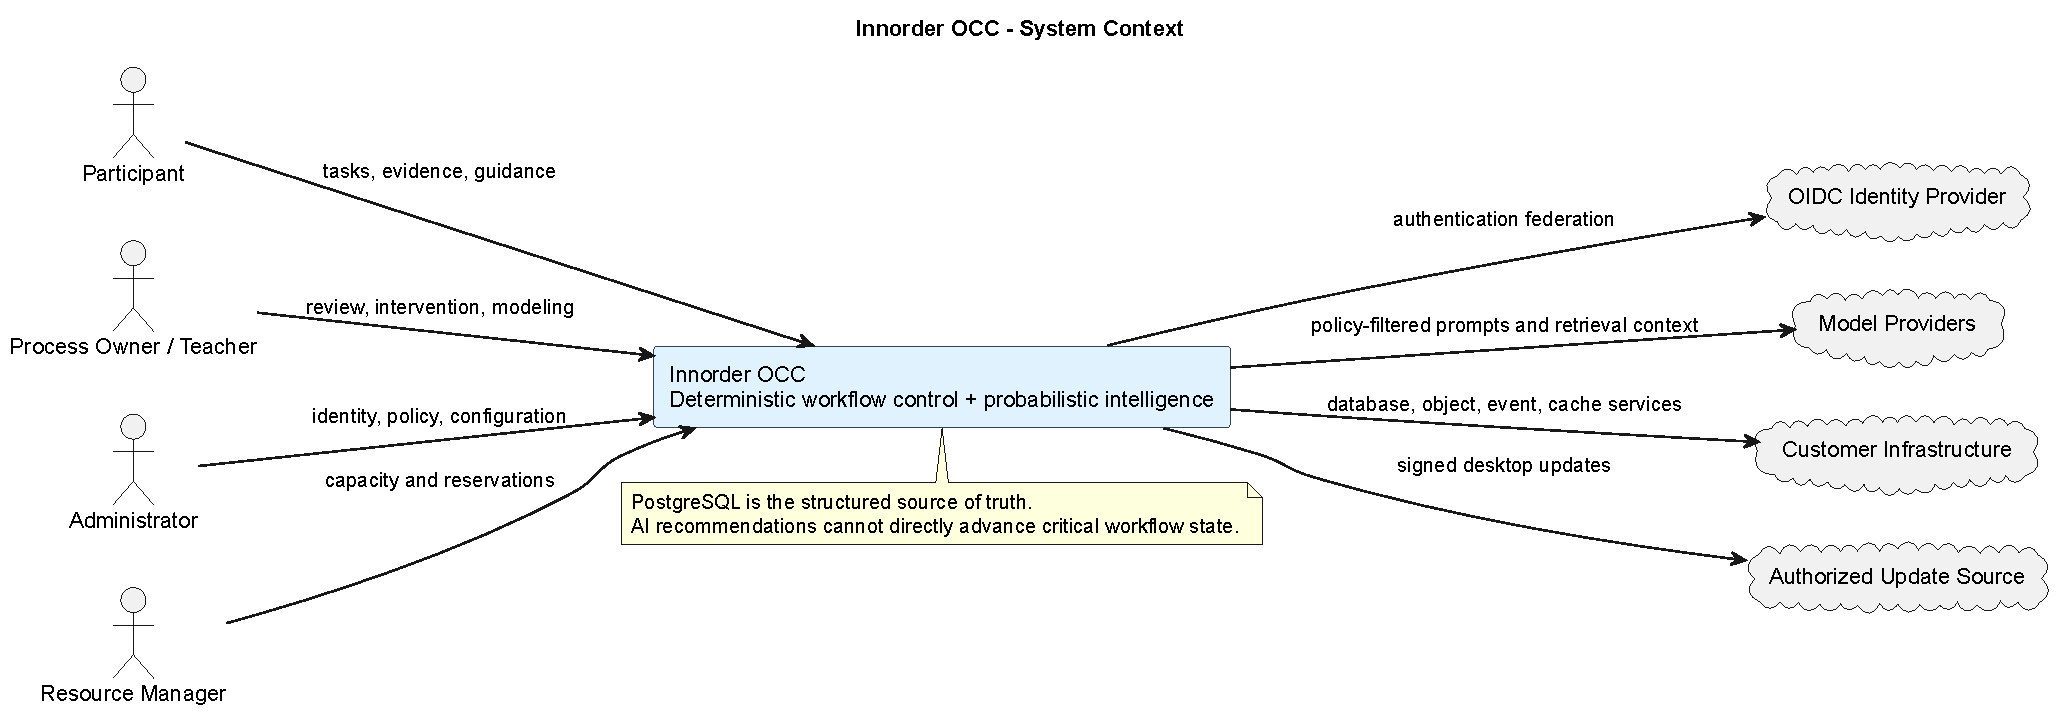
\includegraphics[width=0.98\textwidth]{01-system-context.pdf}
\caption{System context and external trust boundaries.}
\label{fig:context}
\end{figure}

\section{Architecture Specification}
\subsection{System structure}
The target system comprises an Electron desktop client, a Kotlin/Spring Boot modular-monolith Core with embedded Flowable, a separate Node.js/Fastify/LangChain.js AI Service, and PostgreSQL, OPA, Kafka, Redis, and S3-compatible storage. Each customer receives a private deployment. Electron uses domain APIs rather than native Flowable APIs. The AI Service accesses restricted Core APIs, authorized events, and AI-owned database objects. Event consumers cannot directly advance critical Flowable state.

\begin{figure}[H]
\centering
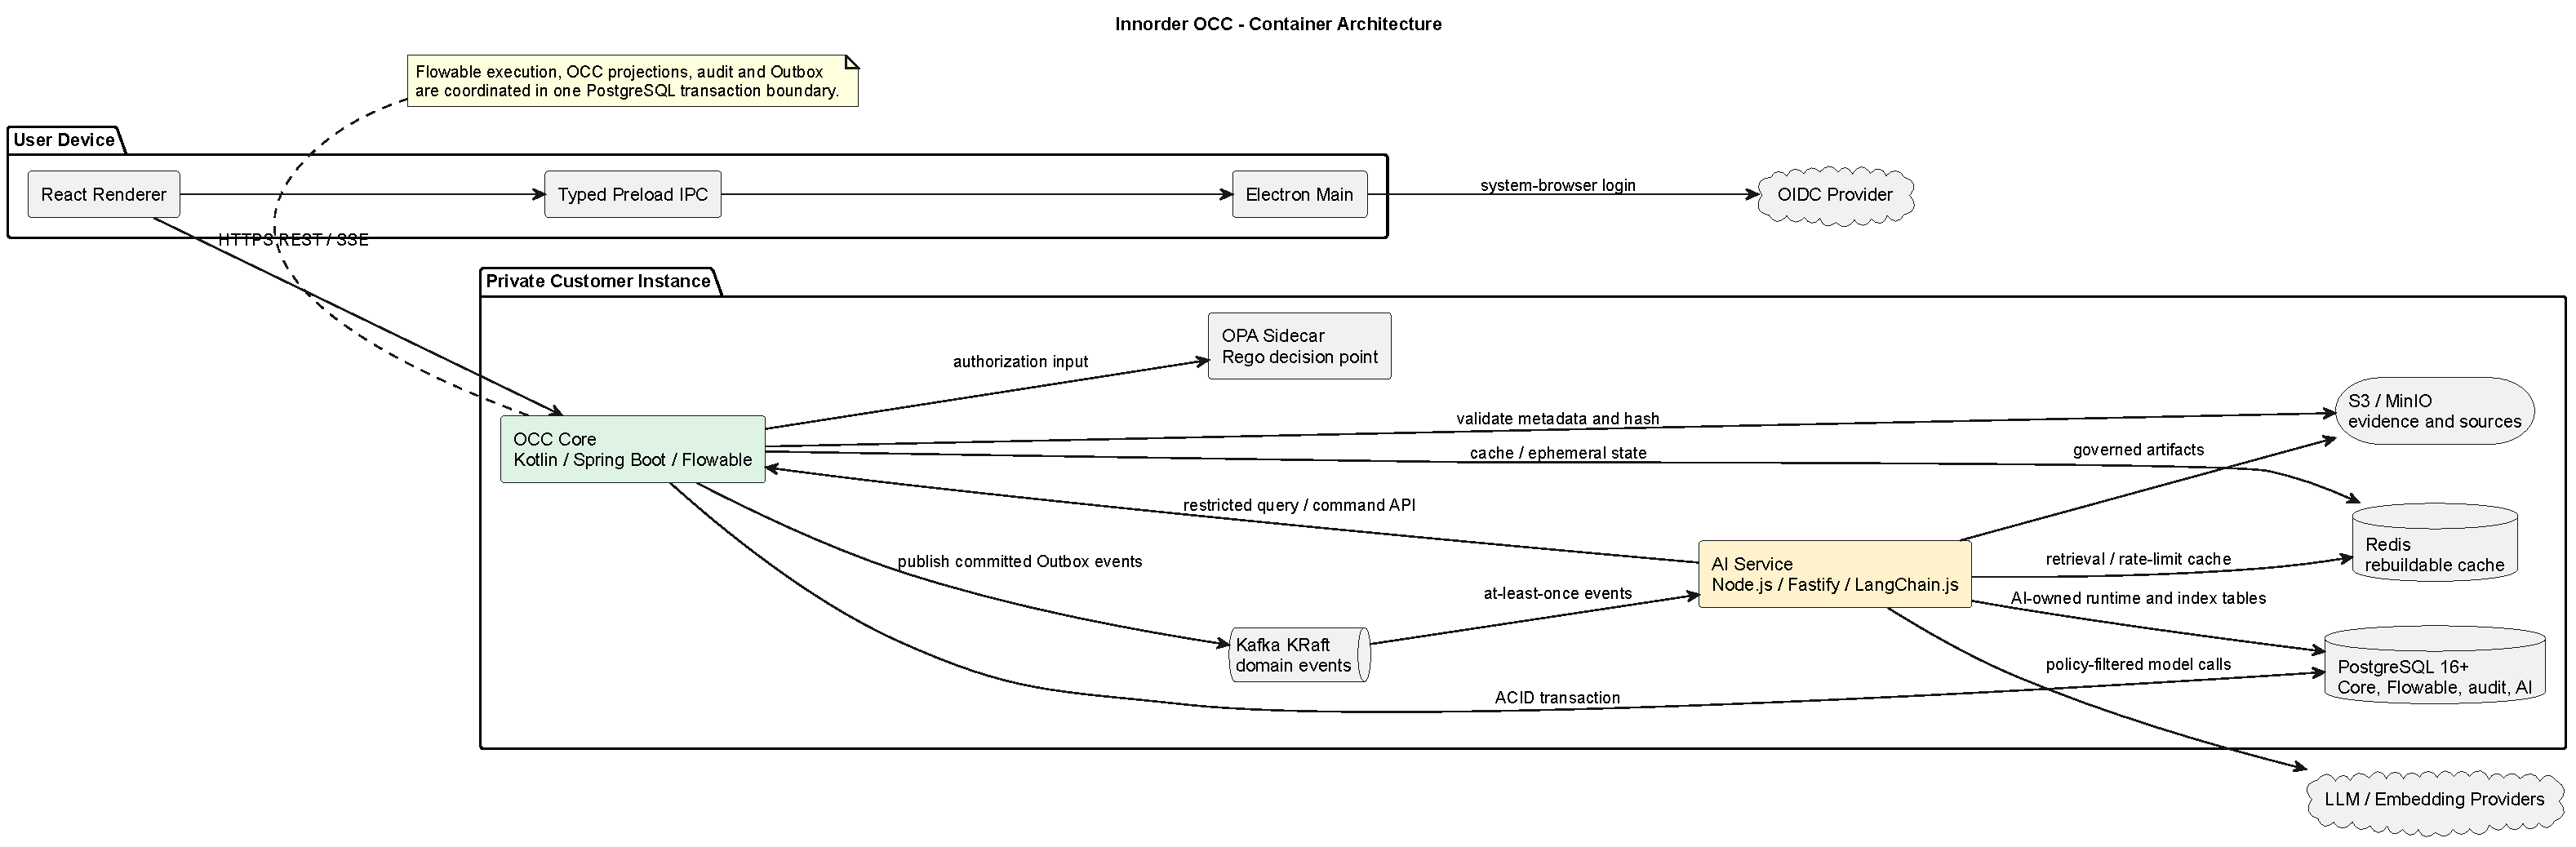
\includegraphics[width=\textwidth]{02-container-architecture.pdf}
\caption{Container architecture and synchronous/asynchronous communication.}
\label{fig:containers}
\end{figure}

\subsection{Architectural invariants}
\begin{enumerate}[leftmargin=*]
\item PostgreSQL is the sole authority for structured business facts. Kafka is not a fact store, and Redis contents must be disposable and reconstructable.
\item Core coordinates Flowable changes, OCC projections, authorization relations, audit, and Outbox records in one database transaction.
\item An object becomes valid evidence only after Core verifies existence, type, size, and SHA-256 and commits evidence metadata.
\item OPA is a stateless decision point; PostgreSQL owns identities, direct relations, authorized attributes, and policy-release metadata.
\item Every applicable DENY overrides ALLOW. No match, OPA failure, or revision mismatch results in denial.
\item AI output remains a recommendation or human queue item and cannot bypass BPMN, DMN, evidence requirements, or approval gates.
\item Domain packages cannot contain arbitrary executable code, DDL, or secrets. Service tasks reference preregistered controlled capabilities.
\end{enumerate}

\subsection{Core module boundaries}
\begin{figure}[H]
\centering
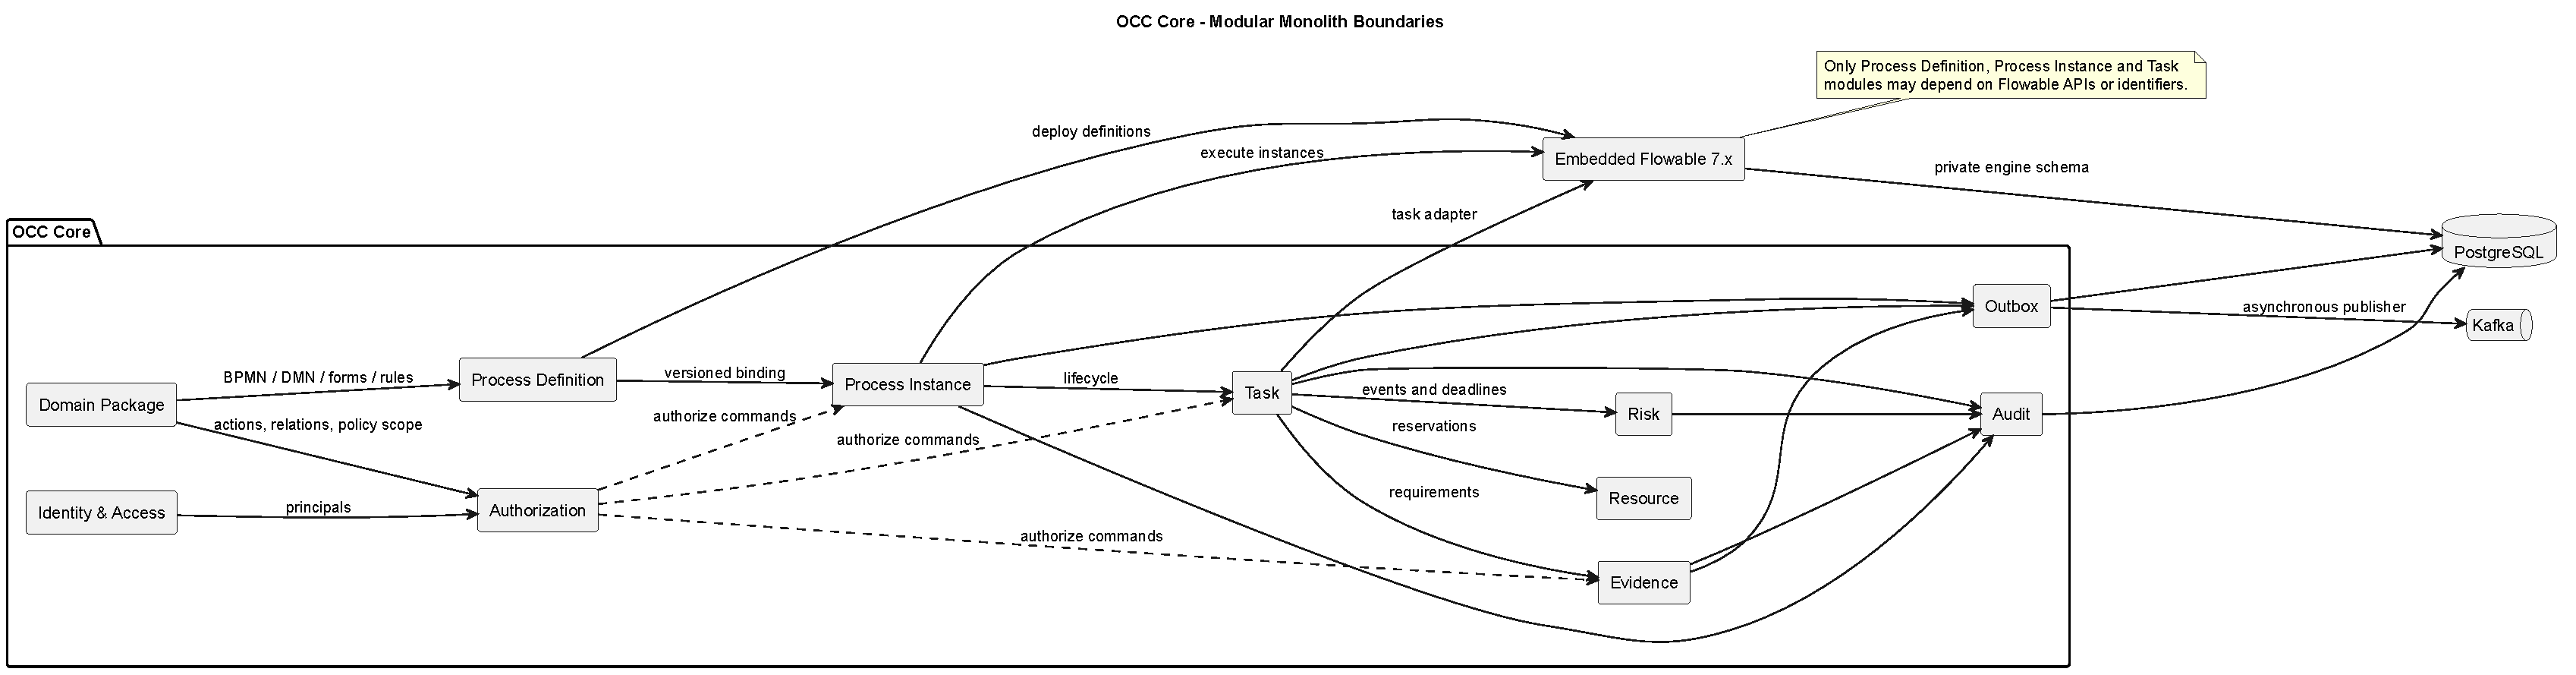
\includegraphics[width=0.94\textwidth]{03-core-modules.pdf}
\caption{OCC Core modular-monolith boundaries and Flowable encapsulation.}
\label{fig:modules}
\end{figure}
Only Process Definition, Process Instance, and Task modules may depend on Flowable APIs or engine identifiers. Other modules collaborate through internal domain interfaces and never query private Flowable tables. Identity \& Access owns authenticating principals; Authorization constructs transaction-snapshot policy input; Domain Package owns versioned assets; Evidence, Risk, Resource, Audit, and Outbox own their corresponding facts.

\section{Functional Requirements}
\subsection{Identity and authorization}
\begin{longtable}{p{0.13\textwidth}p{0.67\textwidth}p{0.12\textwidth}}
\toprule
ID & Requirement & Enforcement \\
\midrule
\endhead
\req{FR-IAM-01} & The system shall support local user accounts and OIDC identity mappings. Groups and roles shall not authenticate. & Core\\
\req{FR-IAM-02} & Every authorizable principal and resource shall use a stable typed entity identity and optimistic row version. & DDL\\
\req{FR-AZ-01} & An authorization-sensitive write shall lock the authorization revision, load direct relations and the active release in the same transaction snapshot, and call local OPA. & Core/test\\
\req{FR-AZ-02} & Relationship writes shall validate published definitions, endpoint types, cardinality, validity, and optional acyclicity. & DDL\\
\req{FR-AZ-03} & A policy release shall atomically combine PLATFORM, DOMAIN, and CUSTOMER bundle versions, include a platform bundle, and be globally unique while ACTIVE. & DDL/Core\\
\req{FR-AZ-04} & Allowed write decisions shall be audited in the business transaction; denied decisions shall be appended in a separate transaction. & Core\\
\bottomrule
\end{longtable}

\subsection{Domain packages and workflow}
\begin{longtable}{p{0.13\textwidth}p{0.67\textwidth}p{0.12\textwidth}}
\toprule
ID & Requirement & Enforcement \\
\midrule
\endhead
\req{FR-DP-01} & A package version shall describe its manifest, BPMN/DMN references, JSON Schema forms, actions, relations, evidence, risk, and knowledge configuration. & Catalog/API\\
\req{FR-DP-02} & Package versions shall follow DRAFT, VALIDATED, PUBLISHED, and DEPRECATED states. Published content shall have a SHA-256 digest and be immutable. & DDL\\
\req{FR-DP-03} & Publication shall validate syntax, references, forbidden elements, permissions, regression scenarios, and impact on running instances. & Core\\
\req{FR-WF-01} & Every process instance shall explicitly bind a package version and Flowable definition binding; a new release shall not implicitly migrate it. & DDL/Core\\
\req{FR-WF-02} & State-changing commands shall use an idempotency key and expectedVersion. Hash mismatch or optimistic-lock conflict shall return HTTP 409. & Core\\
\req{FR-WF-03} & Human tasks shall support creation, claim, completion, cancellation, and failure; assignment and candidacy shall be represented as relationships. & Core/API\\
\req{FR-WF-04} & Flowable state, OCC projections, audit records, and Outbox events shall commit atomically. & Integration gate\\
\bottomrule
\end{longtable}

\subsection{Evidence, risk, and resources}
\begin{longtable}{p{0.13\textwidth}p{0.67\textwidth}p{0.12\textwidth}}
\toprule
ID & Requirement & Enforcement \\
\midrule
\endhead
\req{FR-EV-01} & The client shall upload through a short-lived session; Core shall create an immutable evidence version only after object verification. & DDL/Core\\
\req{FR-EV-02} & Evidence shall bind at least a task or business object and satisfy the applicable type, size, count, and acceptance requirement. & DDL/Core\\
\req{FR-EV-03} & Reviews shall be append-only and support ACCEPTED, REJECTED, and CONDITIONAL decisions with reviewer, reason, and conditions. & DDL\\
\req{FR-RI-01} & A risk shall preserve rule, target, INFO/YELLOW/RED severity, state, confidence, reason, deadline, and resolution time. & DDL\\
\req{FR-RS-01} & Active exclusive reservations shall not overlap for a resource. Capacity reservations shall be checked while holding a resource-row lock. & DDL/Core\\
\bottomrule
\end{longtable}

\subsection{AI, RAG, and collaboration}
\begin{longtable}{p{0.13\textwidth}p{0.67\textwidth}p{0.12\textwidth}}
\toprule
ID & Requirement & Enforcement \\
\midrule
\endhead
\req{FR-AI-01} & The AI Service shall support planning, tutoring, verification, risk, and supervision roles with shared governed tools, traces, and evaluation. & AI Service\\
\req{FR-AI-02} & A model profile shall declare capability, data policy, timeout, rate limit, and cost. Missing required capability shall fail closed. & DDL/AI\\
\req{FR-AI-03} & Tool calls shall use structured schemas, explicit grants and constraints, a required action, and a referenced OPA decision log. & DDL/contract\\
\req{FR-RAG-01} & Retrieval shall authorize document IDs before full-text/vector search and reranking within that candidate set. & Security test\\
\req{FR-RAG-02} & At most one embedding space may be ACTIVE. A replacement shall switch atomically only after coverage and retrieval evaluation gates. & DDL/AI\\
\req{FR-AI-04} & A recommendation shall record its run, target, structured payload, confidence, review state, and versioned citations. Acceptance remains an ordinary authorized command. & DDL/Core\\
\req{FR-AI-05} & Messages, prompts, knowledge, citations, tool calls, and evaluation versions shall remain traceable, and generated content shall be marked. & DDL/UI\\
\bottomrule
\end{longtable}

\section{Domain Model and Lifecycles}
\begin{figure}[H]
\centering
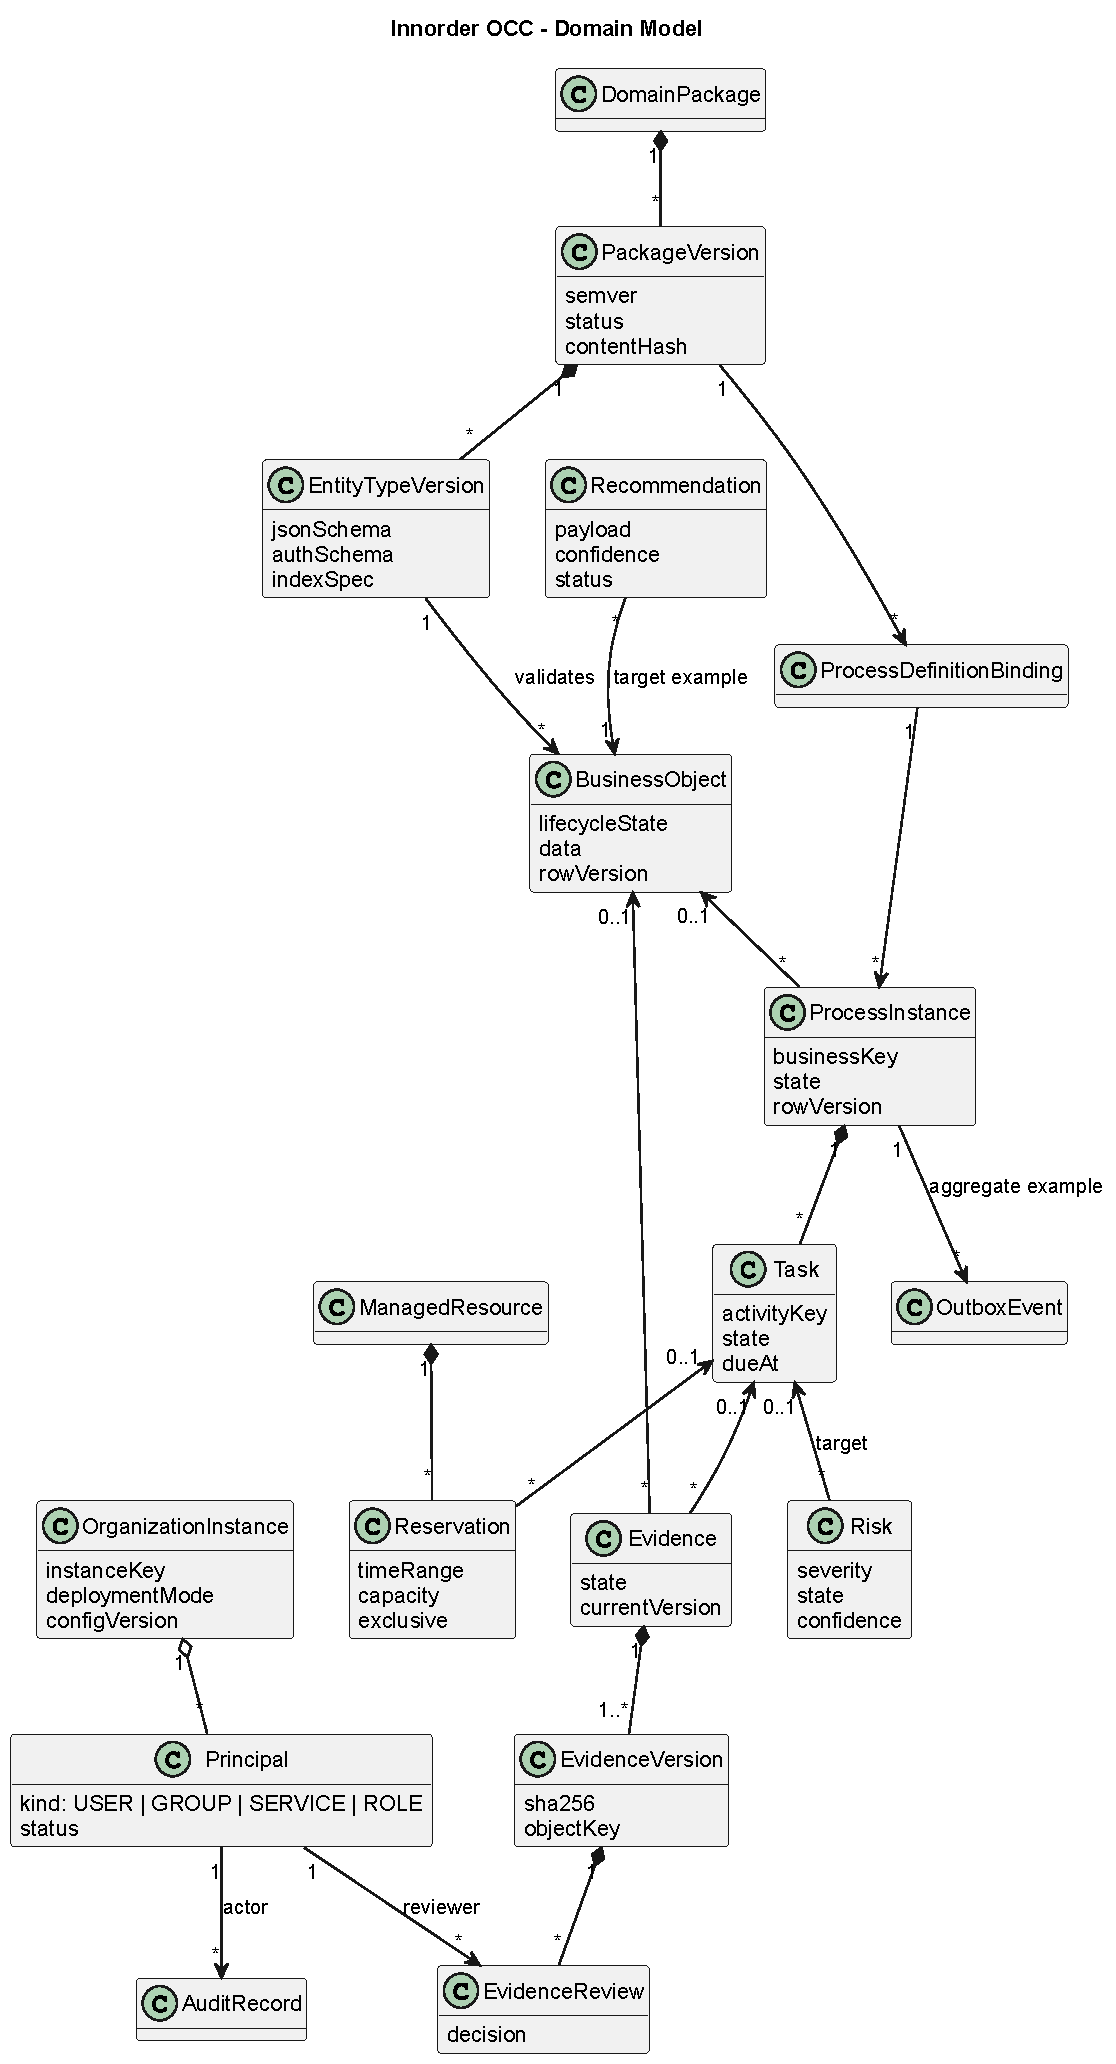
\includegraphics[width=\textwidth,height=0.74\textheight,keepaspectratio]{04-domain-model.pdf}
\caption{Stable domain concepts and aggregate relationships.}
\label{fig:domain}
\end{figure}

\subsection{Aggregate boundaries}
A domain package and its versioned definitions form a publication aggregate. A business object is the extensible domain-data aggregate. Process instances and tasks are OCC-authorizable projections of Flowable state. Evidence consists of a mutable head, immutable versions, and append-only reviews. Risks and reservations represent intervention and resource-use aggregates. An AI run is execution trace data, while a recommendation is an authorizable and reviewable business proposal.

\subsection{Key lifecycles}
\begin{longtable}{p{0.25\textwidth}p{0.60\textwidth}}
\toprule
Object & States and invariants \\
\midrule
\endhead
Package Version & DRAFT $\rightarrow$ VALIDATED $\rightarrow$ PUBLISHED $\rightarrow$ DEPRECATED; published content is immutable.\\
Process Instance & RUNNING/SUSPENDED $\rightarrow$ COMPLETED/CANCELLED/FAILED; terminal state requires ended\_at.\\
Task Projection & CREATED $\rightarrow$ CLAIMED $\rightarrow$ COMPLETED, or CANCELLED/FAILED; completion requires completed\_at.\\
Evidence & PENDING $\rightarrow$ SUBMITTED $\rightarrow$ ACCEPTED/REJECTED, optionally ARCHIVED; current version uses a deferred FK.\\
Risk & OPEN $\rightarrow$ ACKNOWLEDGED $\rightarrow$ RESOLVED/DISMISSED; RESOLVED requires resolved\_at.\\
Policy Release & Inserted only as STAGED, then ACTIVE/RETIRED/FAILED; ACTIVE is globally unique.\\
Embedding Space & BUILDING $\rightarrow$ ACTIVE $\rightarrow$ RETIRED, or FAILED; ACTIVE is globally unique.\\
Recommendation & PROPOSED $\rightarrow$ ACCEPTED/REJECTED/EXPIRED/WITHDRAWN.\\
\bottomrule
\end{longtable}

\section{Critical Interactions and Transactions}
\subsection{Authorization-sensitive command}
\begin{figure}[H]
\centering
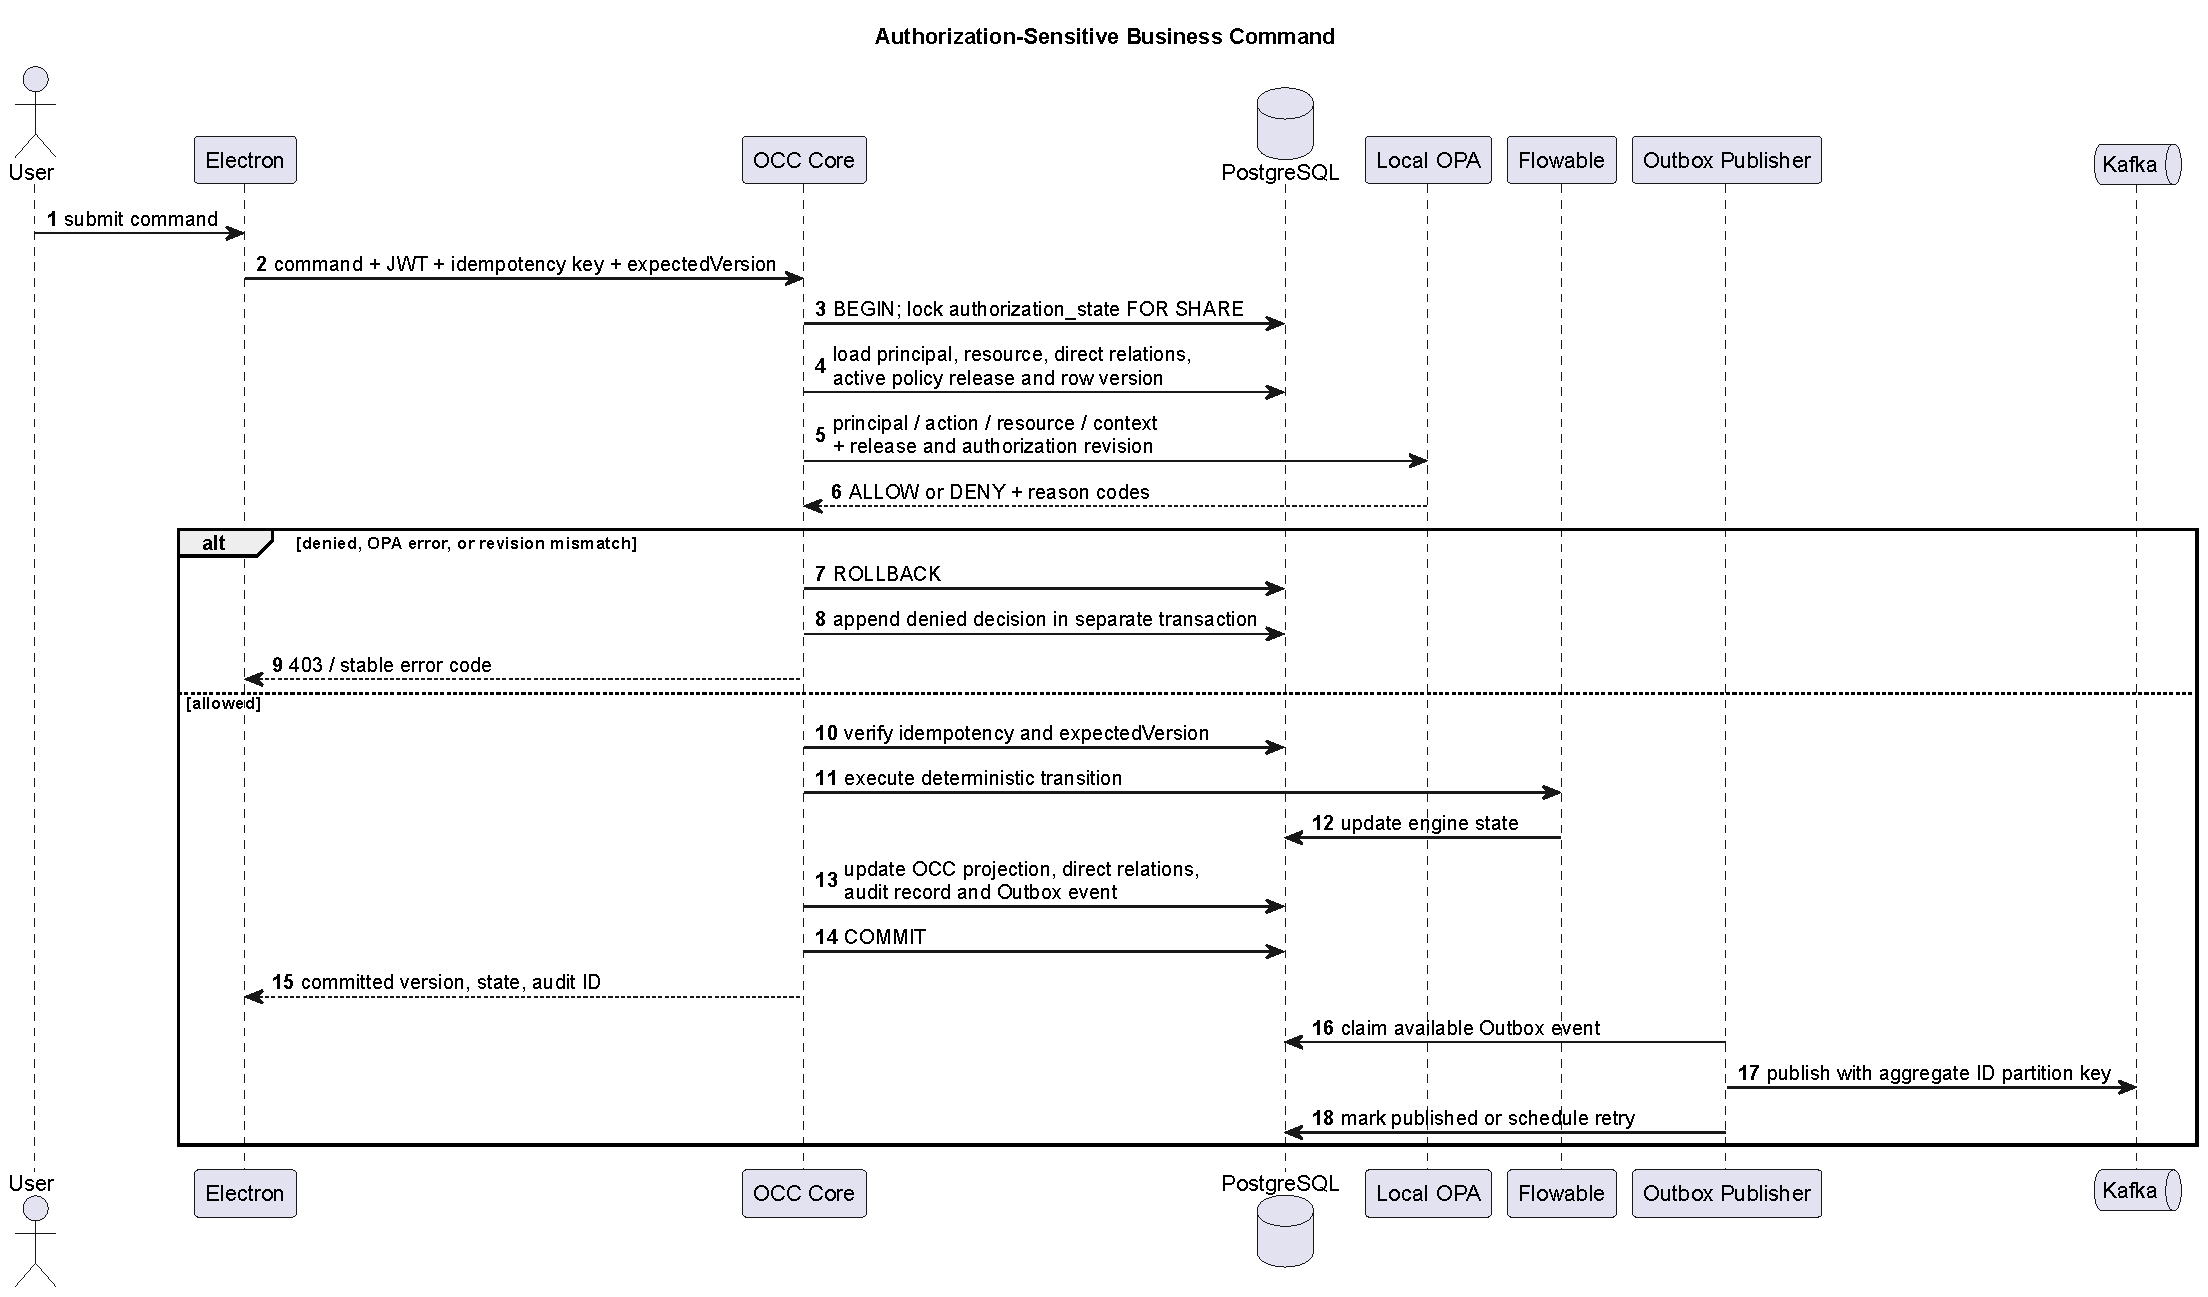
\includegraphics[width=0.90\textwidth]{05-command-transaction-sequence.pdf}
\caption{Authorization, optimistic locking, Flowable, audit, and Outbox order.}
\label{fig:command}
\end{figure}
A normal business write obtains a shared lock on \texttt{authz.authorization\_state}. A relation, policy release, authorization attribute, or entity authorization-state change obtains an exclusive lock and increments the revision. Core sends the locked revision and policy release to OPA and rejects mismatched results. Kafka delivery is at least once; consumers deduplicate by event ID and partition by aggregate ID to preserve aggregate-local order.

\subsection{Evidence submission and review}
\begin{figure}[H]
\centering
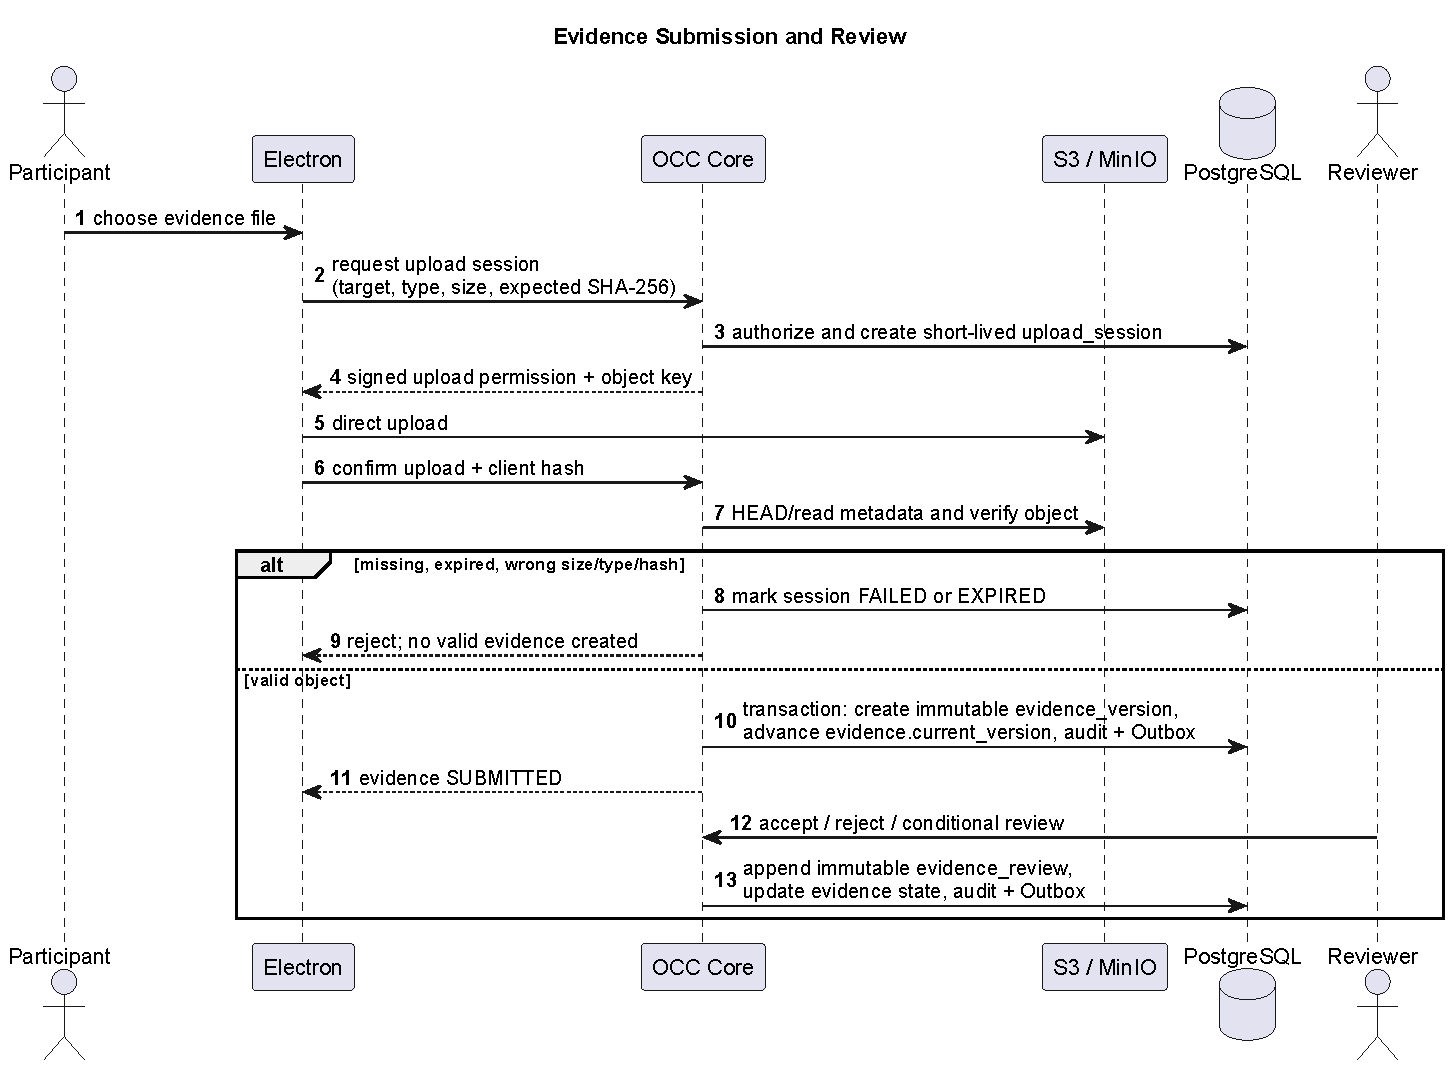
\includegraphics[width=0.88\textwidth]{06-evidence-flow.pdf}
\caption{Evidence lifecycle from temporary object upload to review.}
\label{fig:evidence}
\end{figure}

\section{API and Event Contracts}
REST/OpenAPI is the synchronous contract source for Electron, Core, and AI. Commands carry JWT, \texttt{Idempotency-Key}, \texttt{expectedVersion}, and correlation ID. Errors use Problem Details with a stable code, retryability, correlation ID, and user-readable detail. Domain APIs must not expose native Flowable table names, entities, or internal state codes. SSE carries real-time notifications, but reliable notifications are persisted before delivery.

Kafka JSON envelopes include event ID, schema version, customer instance ID, aggregate type/ID/version, event type, occurrence time, correlation ID, and data classification. CI shall enforce declared compatibility policy. PostgreSQL-to-Kafka exactly-once delivery is explicitly not promised; the model is transactional Outbox, at-least-once publication, aggregate-local ordering, and idempotent consumption.

\section{Security, Privacy, and Governance}
\begin{enumerate}[leftmargin=*]
\item The Electron renderer enables sandbox, context isolation, and CSP and disables Node integration. The main process protects tokens in OS secure storage.
\item Services use separate identities, TLS, and least-privilege database accounts. Only external secret references are persisted.
\item Platform DENY rules cannot be overridden. Policy publication requires compilation, tests, approval, signing, OPA load confirmation, and atomic activation.
\item Authorization attributes are restricted by auth-schema allowlists. Provider-specific data policies default-deny model-bound fields and classifications.
\item Retrieved content is untrusted input and cannot expand system instructions, tool grants, authorization, or approval rules.
\item Audit, evidence versions, policy releases, document versions, and messages are protected through append-only or immutable semantics. Retention and legal hold govern deletion.
\item AI output retains model, prompt, package, knowledge, citations, tool calls, cost, and trace metadata.
\end{enumerate}

\section{Non-functional Requirements}
\subsection{Reliability and degradation}
Kafka failure delays consumers while Core commits and retains Outbox records. Redis failure causes PostgreSQL fallback. AI timeout, rate limiting, malformed output, or missing citations rejects the recommendation or escalates to a person without blocking core commands. Object-store failure cannot create valid evidence. If Core or PostgreSQL is unavailable, Electron offers read-only cached data and disables all writes.

\subsection{Performance baseline}
On a recorded representative private-server configuration, 100 concurrent sessions shall meet: cache-hit query p95 $\leq 200$ ms; PostgreSQL fallback p95 $\leq 500$ ms; state-changing command excluding file and AI p95 $\leq 700$ ms; committed domain event to consumer p95 $\leq 2$ s. Retry and concurrency conflict shall cause no lost or duplicate transition. AI first-token latency, completion latency, failure rate, and cost are reported separately from the Core API SLA.

\subsection{Observability}
All services use structured logs and a common correlation ID. OpenTelemetry covers API, database, Kafka, and model calls. Required metrics include request latency/error rate, Flowable jobs, Outbox backlog, consumer lag, dead letters, Redis hit rate, object upload failure, OPA latency/error, AI token/cost/latency, partition health, and backup status.

\section{Database Design}
\subsection{Platform and scale}
The database baseline is PostgreSQL 16+, UTF-8, with \texttt{vector} and \texttt{btree\_gist}. Current migrations create eight schemas and 70 logical tables plus two default partitions. The \texttt{flowable} schema namespace exists, but vendor engine tables are created and upgraded only by the pinned Flowable release.

\begin{figure}[H]
\centering
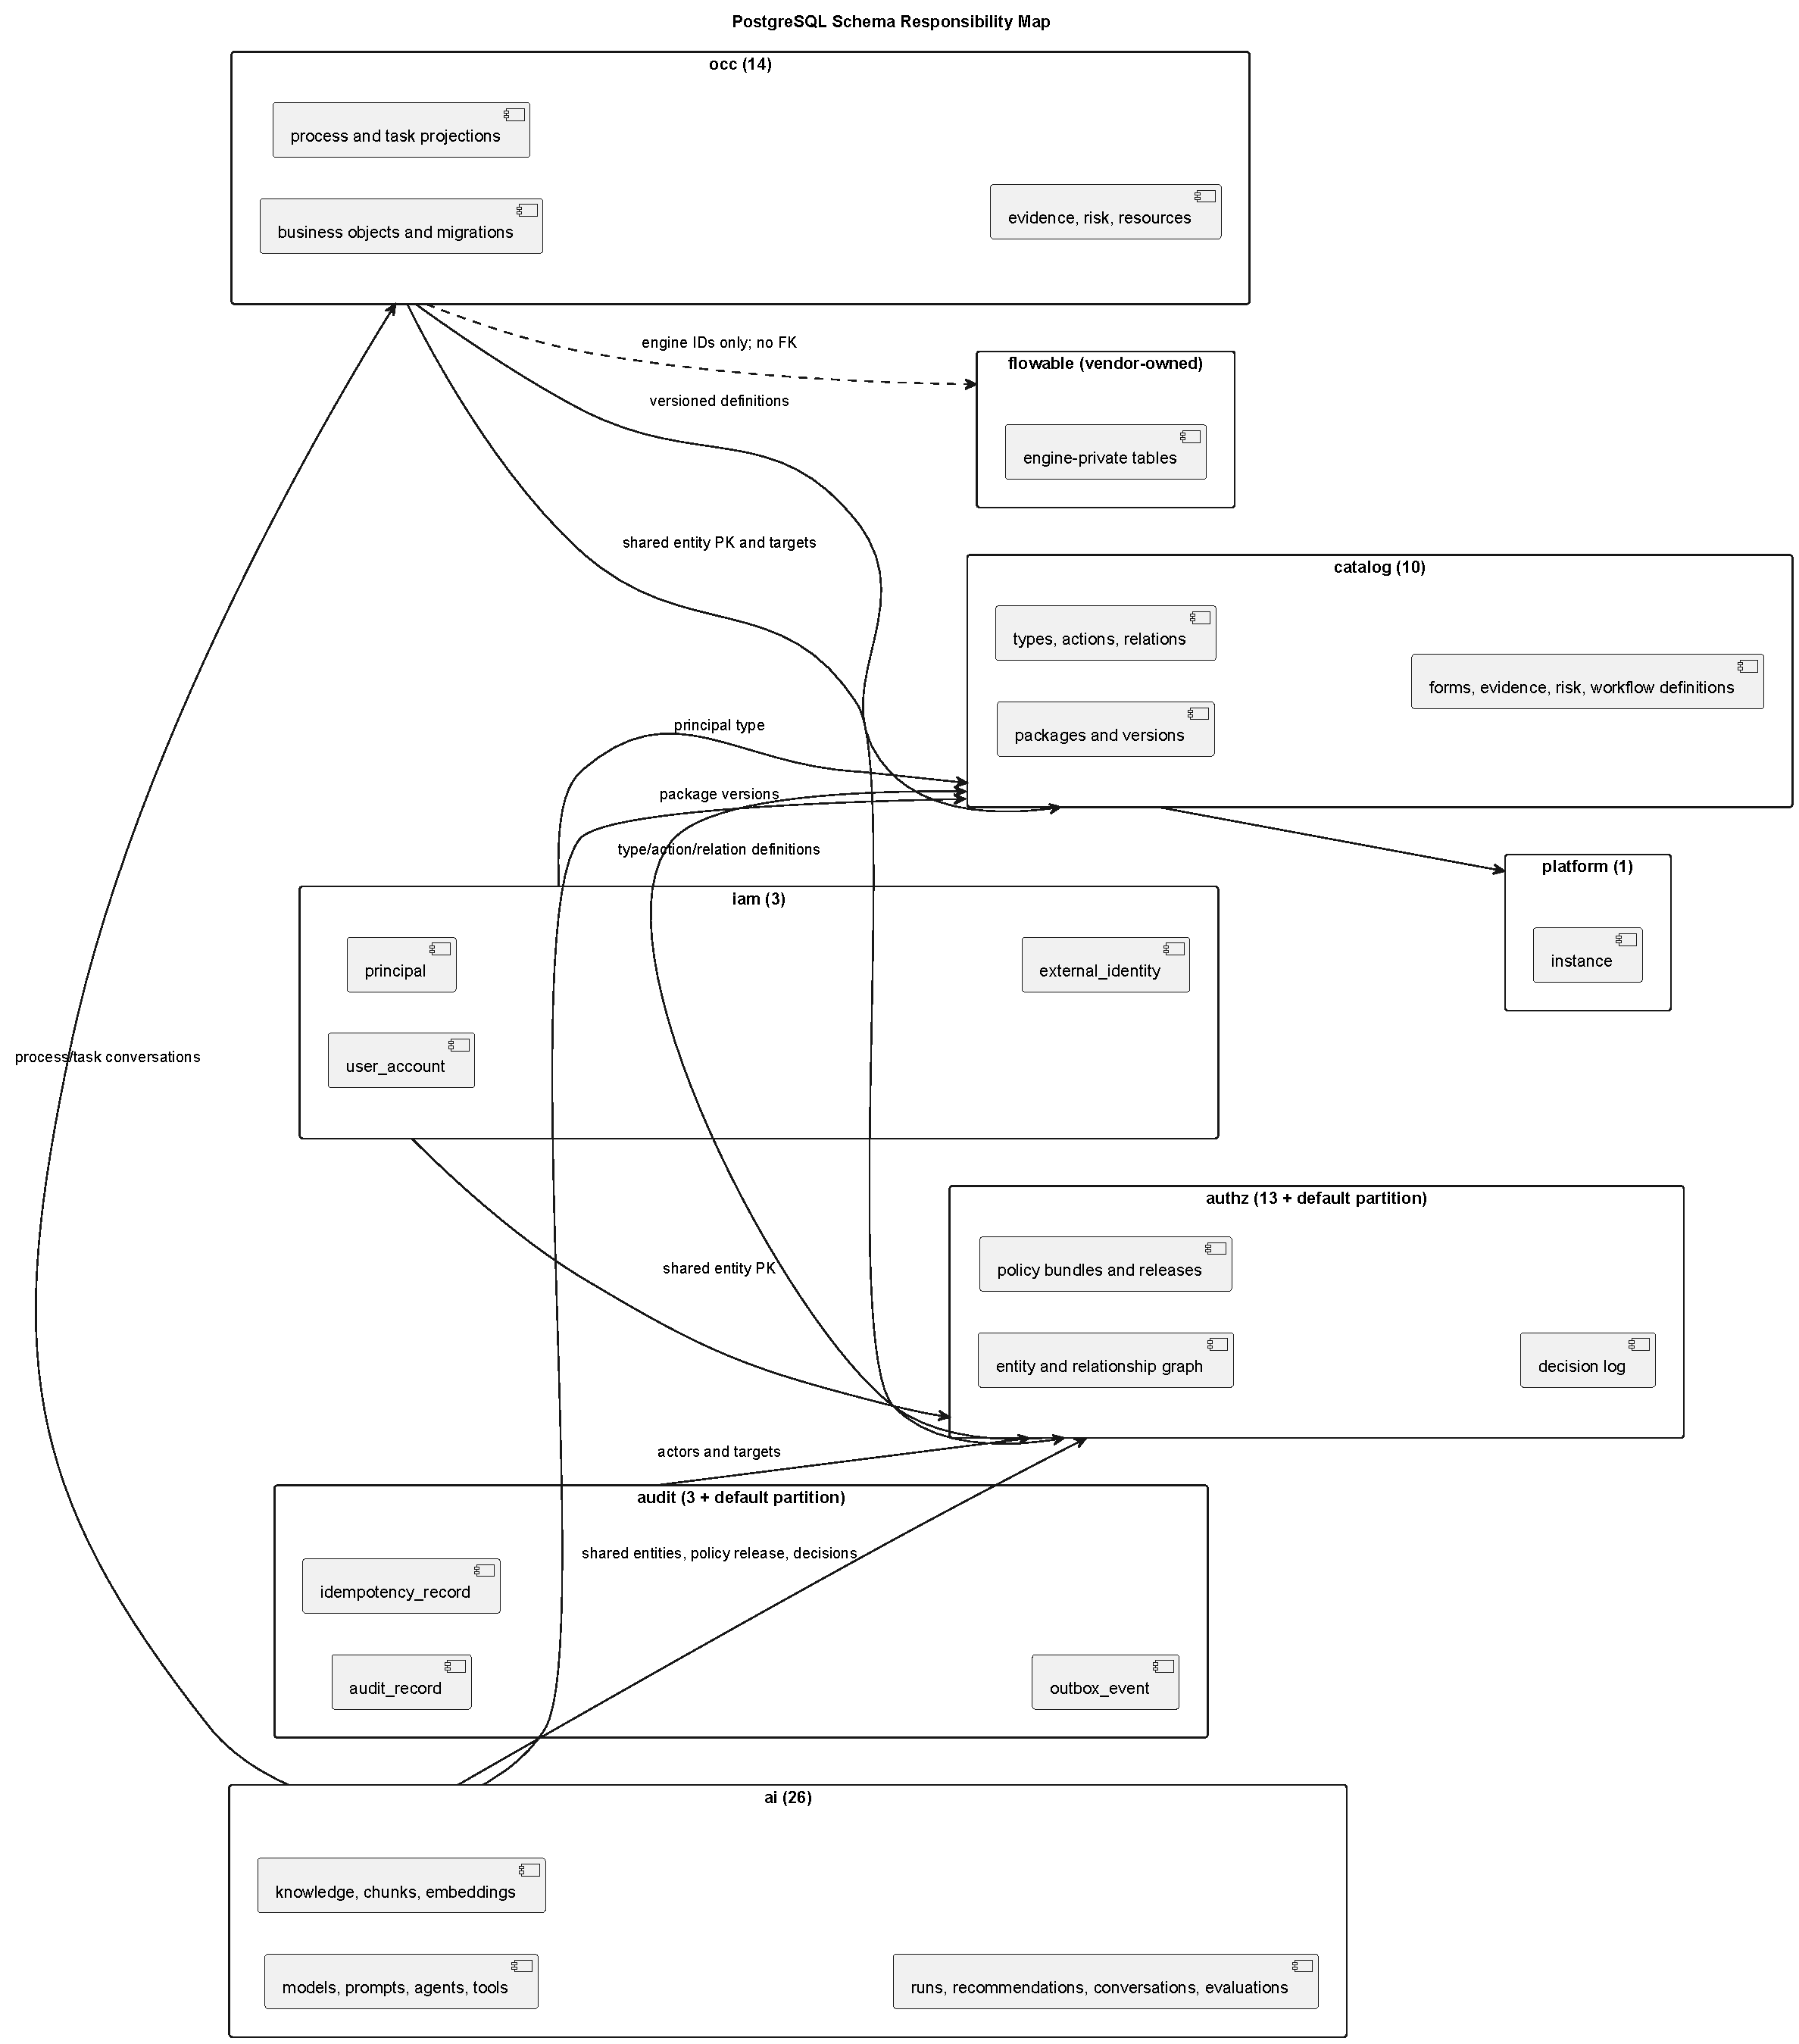
\includegraphics[width=\textwidth]{08-database-schema-map.pdf}
\caption{PostgreSQL schema responsibilities and dependency direction.}
\label{fig:schemas}
\end{figure}

\subsection{Conventions}
Applications generate UUIDv7 keys. Timestamps are UTC \texttt{timestamptz}; monetary values and cost use \texttt{numeric}; extensible states use text plus CHECK rather than PostgreSQL enums. JSON object columns use \texttt{platform.is\_json\_object}. Mutable aggregates use \texttt{row\_version}; update triggers refresh \texttt{updated\_at} and increment the version. Delete defaults to RESTRICT, with CASCADE limited to draft children, rebuildable projections, and tightly owned runtime children.

\subsection{Schema and table inventory}
\begin{longtable}{p{0.12\textwidth}p{0.08\textwidth}p{0.72\textwidth}}
\toprule
Schema & Count & Tables \\
\midrule
\endhead
platform & 1 & instance\\
catalog & 10 & domain\_package, package\_version, entity\_type, entity\_type\_version, action\_definition, relation\_definition, form\_definition, evidence\_requirement, risk\_rule\_definition, workflow\_definition\\
iam & 3 & principal, user\_account, external\_identity\\
authz & 13 & entity, authorization\_state, relationship, relationship\_closure, policy\_bundle, policy\_bundle\_version, policy\_module, policy\_test\_case, policy\_approval, policy\_binding, policy\_release, policy\_release\_item, decision\_log (plus decision\_log\_default)\\
occ & 14 & business\_object, object\_index\_value, data\_migration, data\_migration\_item, process\_definition\_binding, process\_instance, task\_projection, upload\_session, evidence, evidence\_version, evidence\_review, risk, managed\_resource, resource\_reservation\\
audit & 3 & audit\_record, idempotency\_record, outbox\_event (plus audit\_record\_default)\\
ai & 26 & model\_provider, model\_profile, prompt\_template, prompt\_template\_version, agent\_definition, agent\_definition\_version, tool\_definition, agent\_tool\_grant, knowledge\_source, knowledge\_document, knowledge\_document\_version, knowledge\_chunk, embedding\_space, chunk\_embedding, ai\_run, ai\_run\_artifact, tool\_call, recommendation, recommendation\_citation, conversation, message, evaluation\_dataset, evaluation\_dataset\_version, evaluation\_case, evaluation\_run, evaluation\_result\\
flowable & 0 & Vendor-private tables are Flowable-owned; OCC stores engine IDs and defines no cross-boundary foreign keys.\\
\bottomrule
\end{longtable}

\subsection{Unified entity and shared keys}
\texttt{authz.entity} is the authorization supertype. \texttt{iam.principal}, six OCC entities (business object, process instance, task, evidence, risk, and managed resource), and five AI entities (provider, knowledge source/document, recommendation, and conversation) share its primary key. Composite foreign keys align stable entity types with their versions and align a business object with the entity version. Direct relationship facts have a single source in \texttt{authz.relationship}; closure is a rebuildable candidate projection and never an authoritative ALLOW fact.

\begin{figure}[H]
\centering
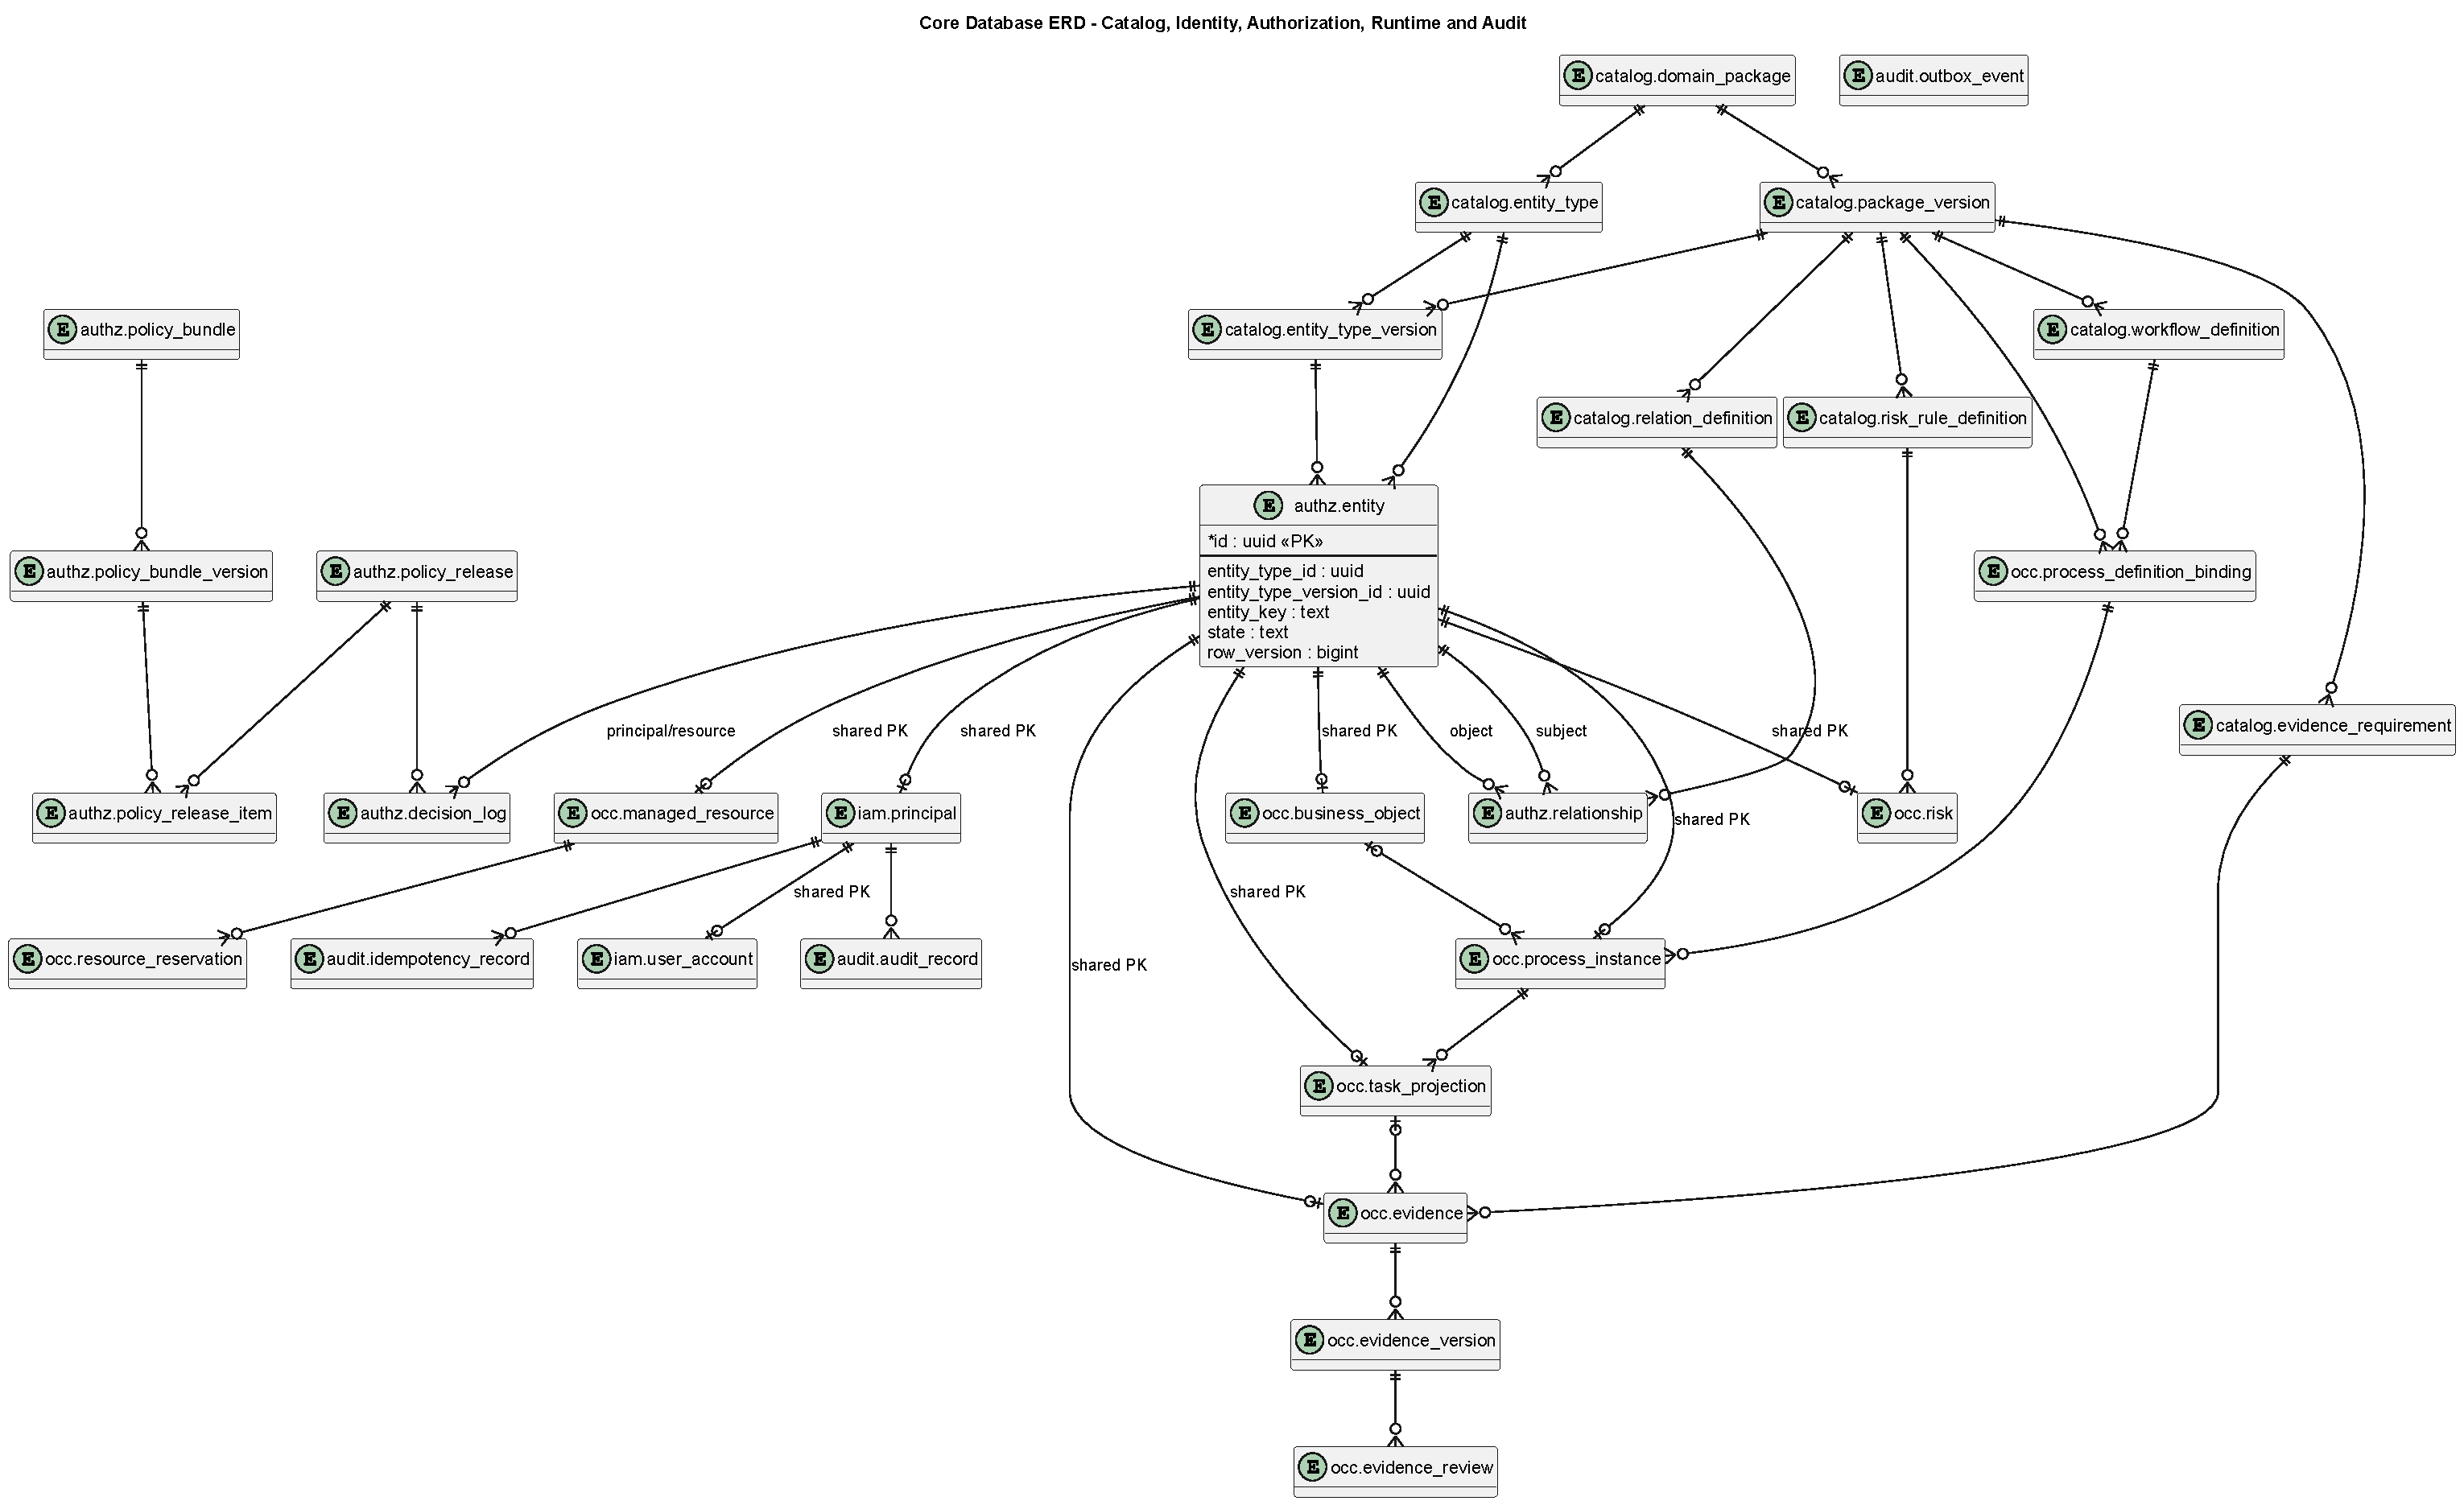
\includegraphics[width=\textwidth]{09-core-database-erd.pdf}
\caption{Core ERD; selected fields and secondary definition tables are omitted for readability.}
\label{fig:coreerd}
\end{figure}

\subsection{Extensible business data}
\texttt{occ.business\_object.data} stores domain fields validated against JSON Schema and remains bound to its creation-time entity-type version. \texttt{object\_index\_value} is a rebuildable typed projection for TEXT, NUMBER, TIMESTAMP, and BOOLEAN filtering, not an EAV source of truth. Explicit data migration and item records track source/target hashes and status; an object changes version only after its item succeeds.

\subsection{Workflow, evidence, and resource integrity}
Flowable deployment, definition, instance, and task identifiers are unique but have no FK to vendor tables. Evidence versions preserve object key, SHA-256, MIME type, and size as immutable facts; a deferred composite FK guarantees current version belongs to the same evidence. A GiST exclusion constraint prevents overlapping active exclusive reservations. Core remains responsible for aggregate capacity checks while locking the resource row.

\subsection{AI and RAG model}
\begin{figure}[H]
\centering
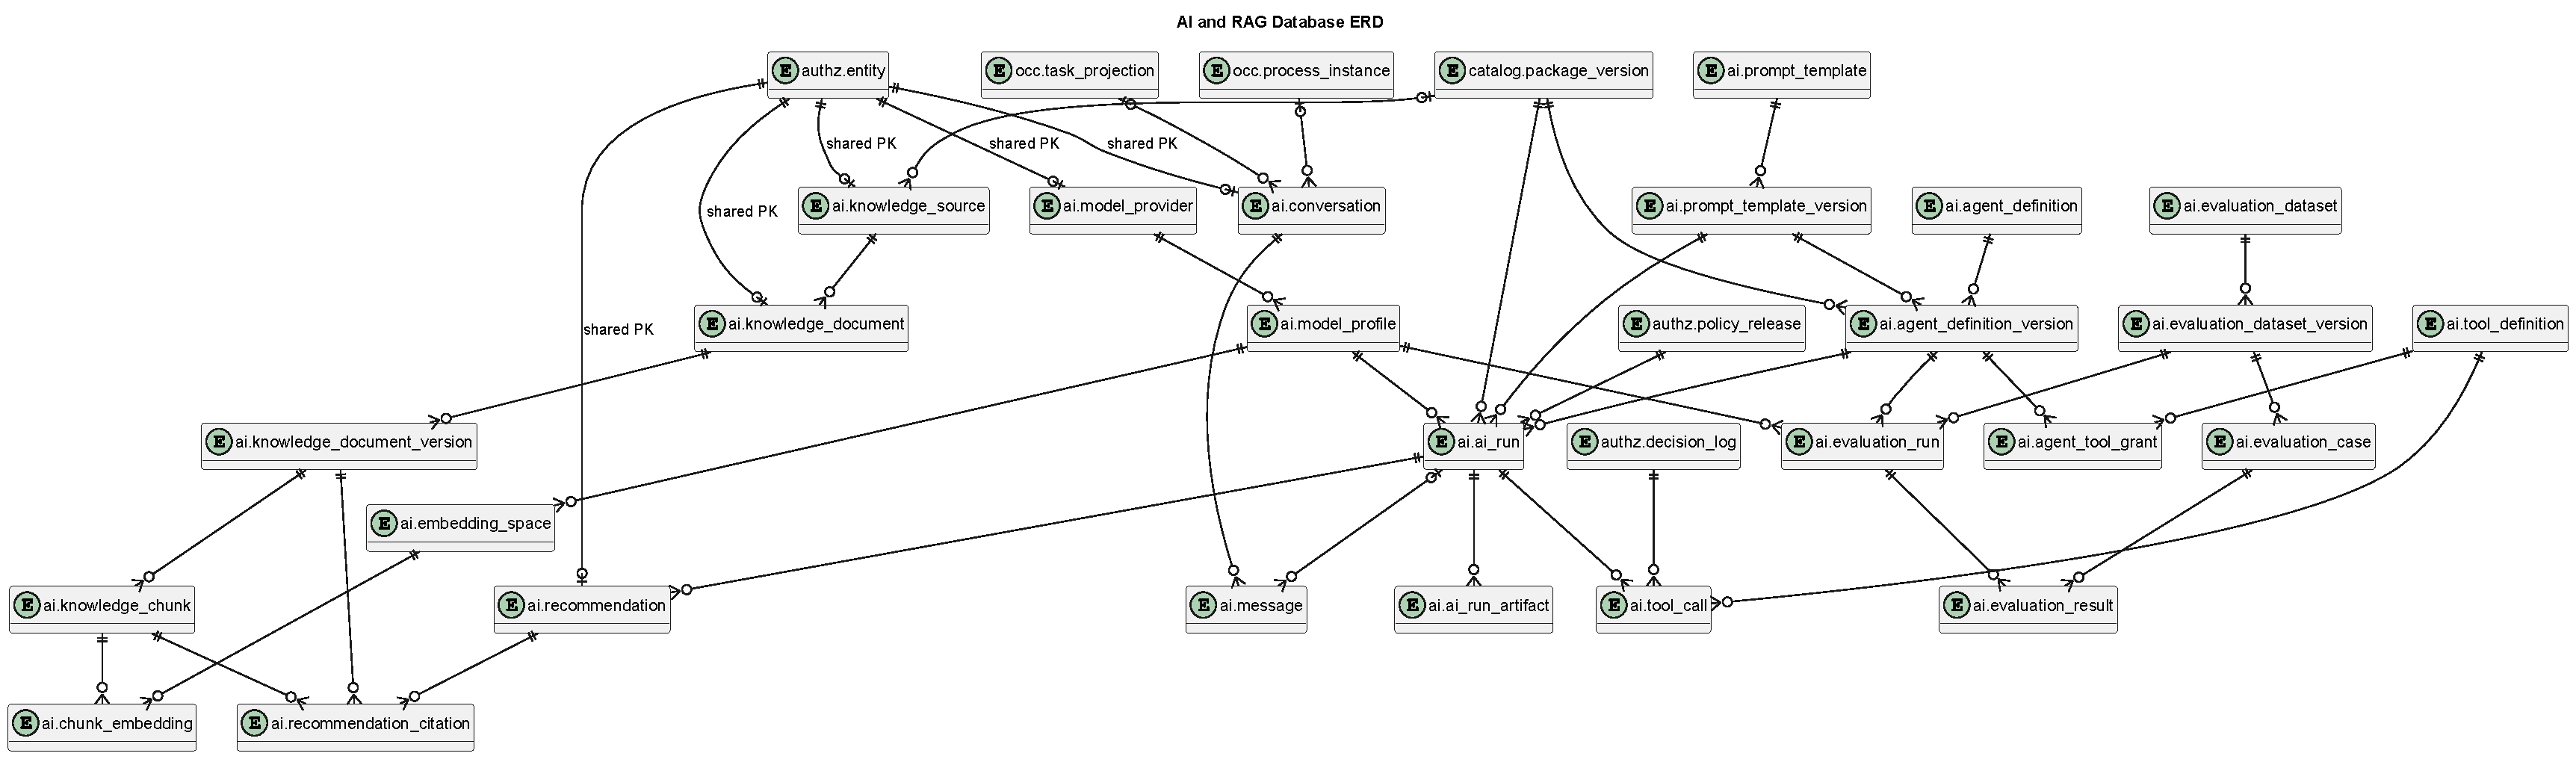
\includegraphics[width=\textwidth]{10-ai-database-erd.pdf}
\caption{AI, RAG, recommendation, conversation, and evaluation ERD.}
\label{fig:aierd}
\end{figure}
Knowledge sources and documents are authorizable entities; chunks inherit document authorization. Full-text search uses a generated \texttt{tsvector} and GIN. Vector data is list-partitioned by embedding space; a helper creates the per-space dimension CHECK and metric-specific COSINE/L2/INNER PRODUCT HNSW index. Tool calls reference partitioned decision logs by (ID, created\_at). A composite citation FK proves that each cited chunk belongs to the declared document version.

\subsection{Indexes, partitions, and immutability}
Indexes cover entity type/state, bidirectional relationship traversal and validity, JSONB business data, typed projection values, task/evidence/risk queues, pending Outbox, knowledge full text, AI runs, and message chronology. Decision and audit logs are range-partitioned with writable default partitions. Chunk embeddings are list-partitioned by space. Operations must create monthly partitions ahead of time and move eligible default-partition rows during maintenance.

\subsection{Database account boundary}
The target deployment has migration, Core, AI, and read-only audit accounts. The AI account cannot read Flowable, credential, or private OCC data and cannot write IAM, authorization, or OCC facts. Current migrations create no roles, grants, restricted views, or RLS, so deployment SQL and privilege regression tests remain a mandatory delivery gate.

\begin{figure}[H]
\centering
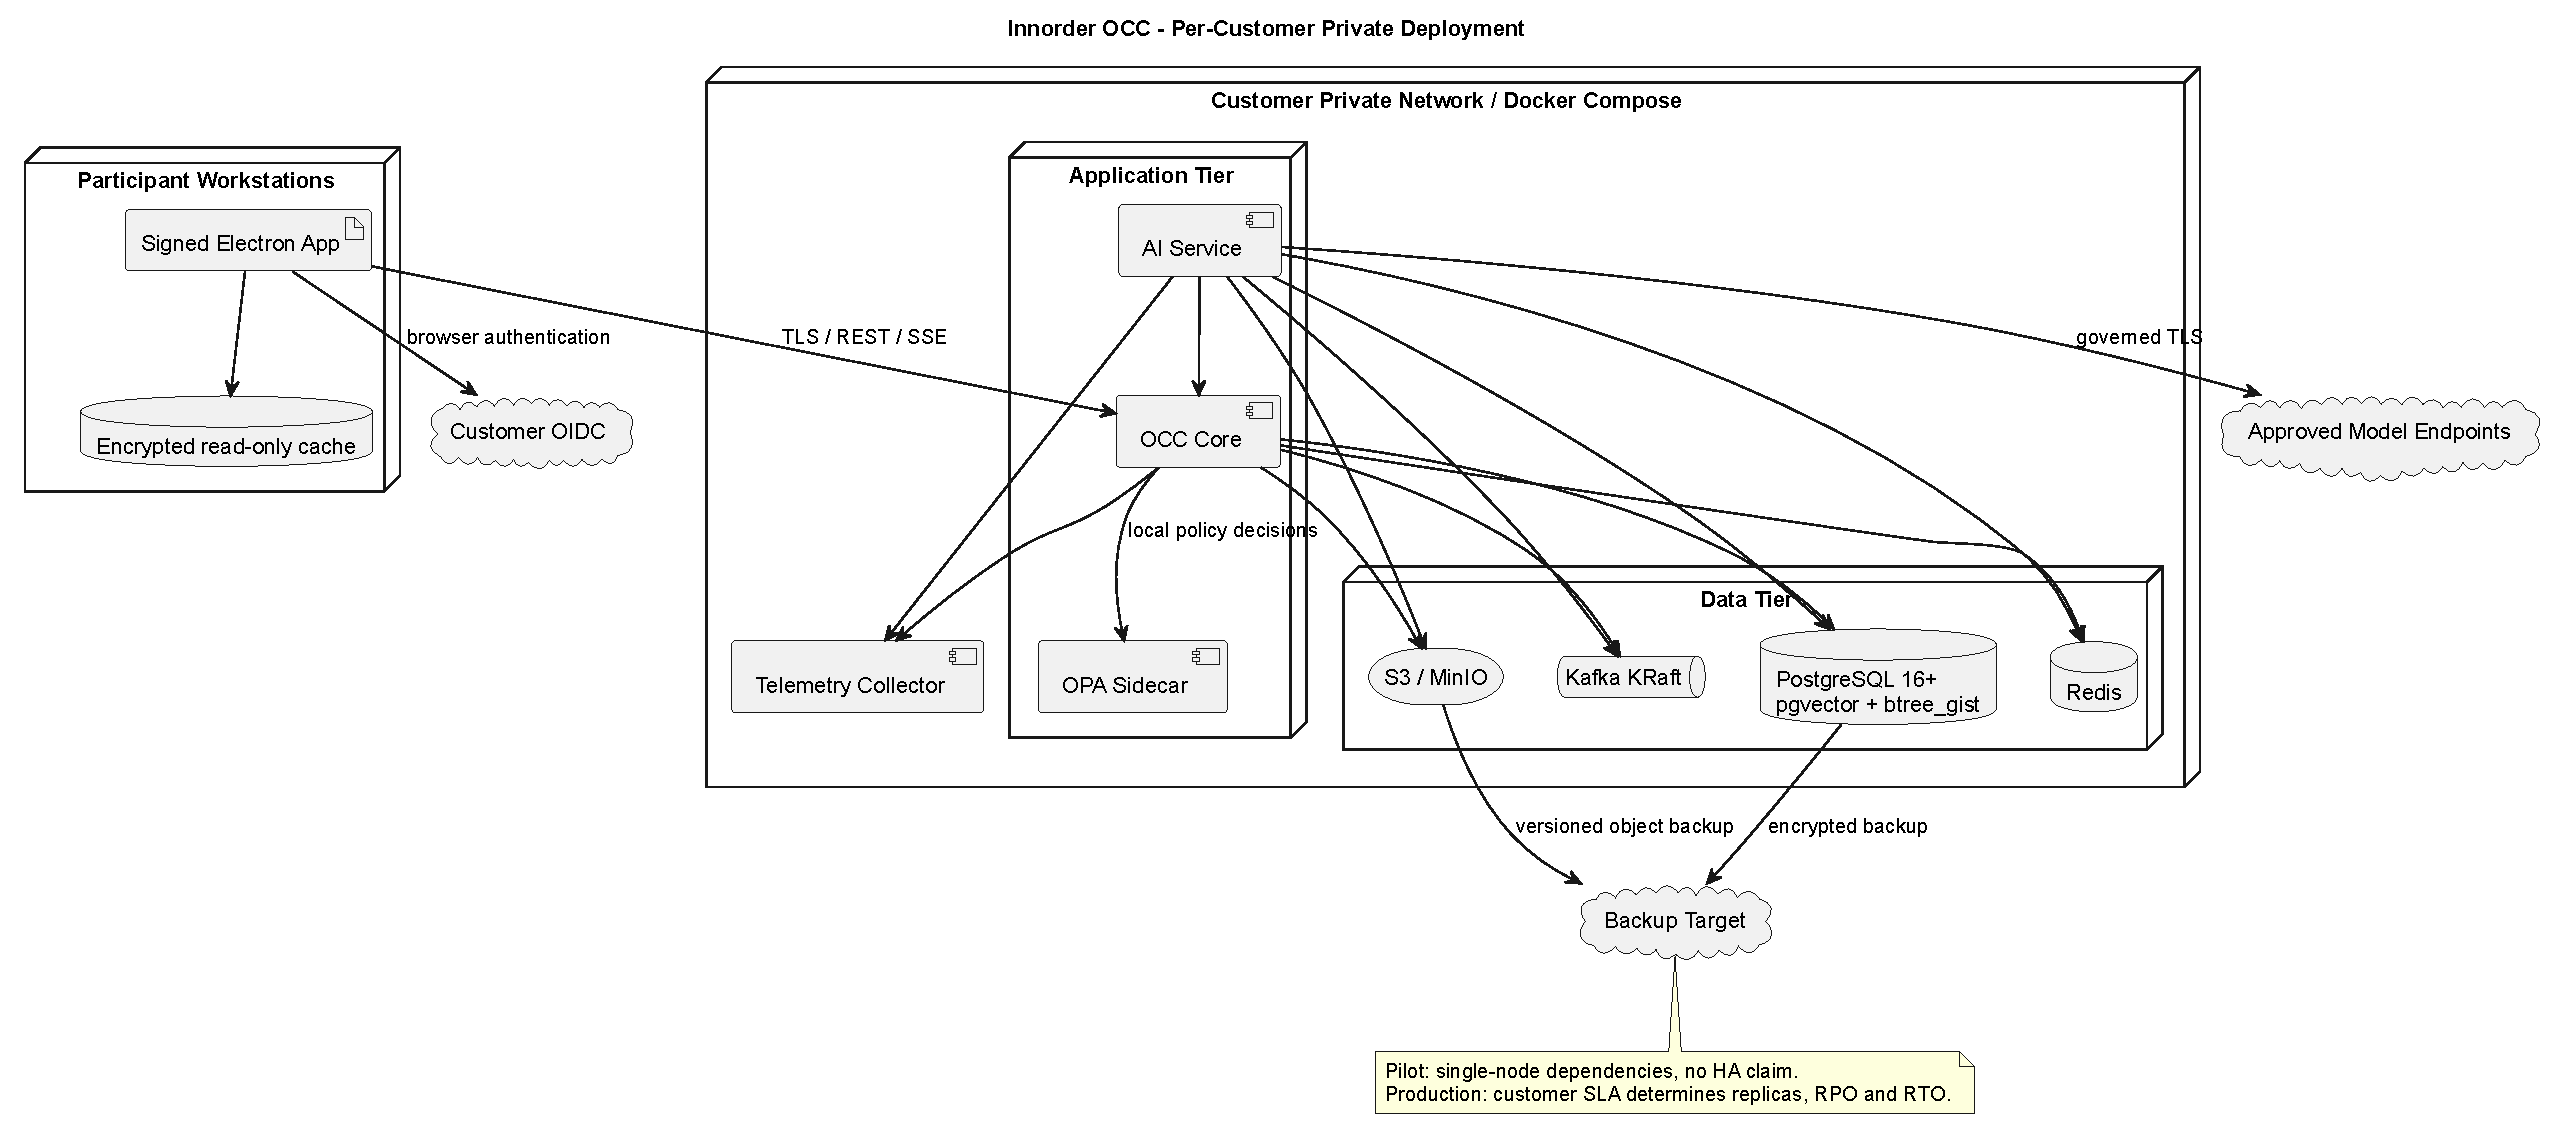
\includegraphics[width=0.95\textwidth]{07-deployment.pdf}
\caption{Per-customer private deployment topology.}
\label{fig:deployment}
\end{figure}

\section{Verification and Acceptance}
\subsection{Existing evidence}
Node static tests verify migration order, absence of placeholders, schemas/extensions, critical tables, authorization/concurrency safeguards, trigger return patterns, cross-table versions, and immutable policy content. SQL contract tests exercise key objects and selected mutation constraints. The README records a successful clean PGlite 0.5.4 run, but PGlite used a compatibility domain in place of pgvector.

\subsection{Release gates}
\begin{enumerate}[leftmargin=*]
\item Apply V001--V008 and all SQL contracts to real PostgreSQL 16 with pgvector.
\item Execute \texttt{ai.create\_embedding\_partition} and verify dimensions, operator class, and HNSW creation.
\item Use Testcontainers to prove Flowable/OCC/audit/Outbox atomicity, Kafka replay, Redis degradation, and object-upload semantics.
\item Test concurrent revocation, policy switch, relationship change, and business writes to exclude TOCTOU authorization bypass.
\item Test default deny, DENY precedence, non-overridable platform DENY, relationship cardinality, and cycle rejection.
\item Prove unauthorized documents never enter RAG candidates and test prompt injection, tool escalation, and uncited output.
\item Execute Electron security, end-to-end, read-only offline, installer signing, upgrade, and rollback tests.
\item Run k6 performance baselines and rehearse backup restore, policy rollback, partition archive, and object cleanup.
\end{enumerate}

\subsection{Pilot outcomes}
For the first 10--20 student pilot: critical-node evidence completeness $\geq95\%$; invalid-skip interception $\geq90\%$; repetitive teacher follow-up time reduced $\geq30\%$; valuable waiting-period task coverage $\geq70\%$; zero missed known severe red risks; risk false-positive rate $\leq20\%$; weekly student activity $\geq80\%$; process changes effective within one business day.

\section{Implementation Gaps and Decisions}
\begin{longtable}{p{0.29\textwidth}p{0.30\textwidth}p{0.33\textwidth}}
\toprule
Topic & Current fact & Required disposition \\
\midrule
\endhead
Service credentials & Design allows USER/SERVICE authentication; DDL only has USER-only user\_account. & Select OIDC client credentials, mTLS, or a controlled new persistence model before implementation.\\
AI run immutability & Design calls AI runs append-only; DDL has no immutable trigger for run, artifact, tool call, or evaluation records. & Define mutable lifecycle columns and freeze terminal records or add history.\\
Monthly partitions & DDL has only audit/decision default partitions, no maintenance helper; AI runs are unpartitioned. & Add operational migration and monitoring; partition AI logs if measured volume warrants it.\\
Least privilege & DDL defines no roles, grants, restricted views, or RLS. & Deliver deployment privilege SQL and regression tests.\\
Shared-PK subtype & Principal and business object types are checked; other shared-PK tables do not prove expected subtype. & Enforce in Core factories or database triggers and test it.\\
Cross-package consistency & Several workflow/binding/instance and agent/prompt/package pairs do not fully prove compatible package ownership. & Reject inconsistent references during publication and add composite FKs where practical.\\
Policy publication gates & DDL does not require all tests and approvals before status publication. & Core publication command must verify compilation, tests, and approval before transition.\\
Real pgvector & PGlite substituted a compatible type and did not verify actual HNSW behavior. & Treat real PostgreSQL/pgvector execution as a non-waivable production gate.\\
\bottomrule
\end{longtable}

\section{Project Document Summary}
The proposal establishes the product thesis: begin with embedded-development education to validate an ``people--task--evidence--resource--risk'' control kernel in a low-liability, repeatable setting, using a 16-week, 10--20 participant pilot. The architecture design turns that thesis into per-customer private deployment, an Electron client for all users, embedded Flowable in a modular Core, a separate AI Service, three-layer OPA policy, Kafka Outbox events, and rebuildable Redis caches. The database design turns cross-domain extensibility into a versioned catalog, unified authorization entities, strong relational cores with JSONB domain data, workflow projections, immutable evidence, explicit data migration, and authorization-first RAG. The SQL migrations implement most of this data foundation and major integrity rules; application services, deployment privileges, real infrastructure integration, and several governance gates remain to be built and verified.

\section{Conclusion}
Innorder OCC places correctness in a deterministic Core and transactional database while constraining AI to traceable, rejectable, human-reviewable recommendations. The current database baseline is sufficient to begin the MVP for domain packages, authorization graph, process projections, evidence, risk, resources, Outbox, and AI/RAG. The next engineering priorities are a Flowable atomic-transaction prototype, OPA revision concurrency tests, database-account isolation, real pgvector verification, and the first teaching domain package, rather than expanding the number of Agents or industries.

\begin{thebibliography}{9}
\bibitem{proposal} Innorder OCC Project Proposal, V1.0, July 2026.
\bibitem{architecture} Innorder OCC Technology Selection and Architecture Design, July 28, 2026.
\bibitem{database} Innorder OCC Database Design, July 28, 2026.
\bibitem{postgres} PostgreSQL Global Development Group, ``PostgreSQL Documentation,'' \url{https://www.postgresql.org/docs/}.
\bibitem{flowable} Flowable, ``Flowable Open Source Documentation,'' \url{https://www.flowable.com/open-source/docs/}.
\bibitem{opa} Open Policy Agent, ``OPA Documentation,'' \url{https://www.openpolicyagent.org/docs/latest/}.
\bibitem{pgvector} pgvector, ``Open-source vector similarity search for Postgres,'' \url{https://github.com/pgvector/pgvector}.
\end{thebibliography}

\end{document}
